\documentclass[12pt,a4paper]{book}
\usepackage[utf8]{inputenc}
\usepackage[inline]{enumitem}
\usepackage{parskip} % disable indentation for new paragraphs, increased margin-bottom instead
\usepackage[american,ngerman]{babel}
\usepackage{csquotes}

\usepackage{kit_style/kitthesiscover}

\usepackage[style=alphabetic]{biblatex}
\addbibresource{bib.bib}

\usepackage[%dvipdfm,
   pdfauthor={Christian Schwarz},
   pdftitle={Stage-aware Scheduling in a Library OS},
   pdfsubject={Bachelor Thesis},
   pdfkeywords={Operating Systems, Library OS, Scheduler, Cache-Affinity}
]{hyperref}

\usepackage{todonotes}
\usepackage{blindtext}

\usepackage{xparse}
\NewDocumentCommand{\sectionsubheading}{m}{%
    {\vspace{-0.7cm}\footnotesize #1 \vspace{0.25em}}\par%
}

\usepackage{xspace}

\usepackage{listings}

% for core allocation pseudo-code mostly...
\usepackage{amsmath}
\usepackage{algorithmicx}
\usepackage{varwidth}
\usepackage{calc} % for \widthof
%\usepackage{algorithm}
\usepackage{algpseudocode}
\usepackage{mathtools}
\DeclarePairedDelimiter\ceil{\lceil}{\rceil}
\DeclarePairedDelimiter\floor{\lfloor}{\rfloor}
\usepackage{amsfonts}
\usepackage{setspace}

% pandas to_latex tables look good this way
\usepackage{booktabs}
\usepackage{multirow}

\usepackage{subcaption}


\lstdefinestyle{figurecpp}{
  belowcaptionskip=1\baselineskip,
  language=C++,
  basicstyle=\footnotesize,
  frame=single,
  xleftmargin=\parindent,
  alsodigit={:},
}

\usepackage{hyperref}
\NewDocumentCommand{\gitcommit}{m}{\texttt{\StrLeft{#1}{8}}}
\NewDocumentCommand{\gitbranch}{m}{\texttt{#1}}
\NewDocumentCommand{\gitrepo}{m}{\texttt{#1}}
\NewDocumentCommand{\refosvcommit}{m}{\href{https://github.com/problame/ba-osv/commit/#1}{\gitcommit{#1}}}

\NewDocumentCommand{\evalfigpath}{m}{fig_build/evaluation/#1}

\widowpenalty100000
\clubpenalty100000
\raggedbottom

\begin{document}
\frontmatter
\unitlength1cm
\selectlanguage{american}

\title{Stage-aware Scheduling in a Library~OS}
\author{cand. inform. Christian Schwarz}
\thesistype{ba}
\primaryreviewer{Prof.\ Dr.\ Frank Bellosa}
\advisor{M.\ Sc.\ Mathias Gottschlag}{}
\thesisbegindate{XX.\ December 2017}
\thesisenddate{XX.\ March 2018}
\maketitle

\begin{otherlanguage}{ngerman}
\thispagestyle{empty}
\vspace*{30\baselineskip}
\hbox to \textwidth{\hrulefill}
\par
\noindent Ich versichere wahrheitsgem"a"s, die Arbeit selbstst"andig verfasst, alle benutzten Hilfsmittel vollst"andig und genau angegeben und alles kenntlich gemacht zu haben, was aus Arbeiten anderer unver"andert oder mit Ab"anderungen entnommen wurde sowie die Satzung des KIT zur Sicherung guter wissenschaftlicher Praxis in der jeweils g"ultigen Fassung beachtet zu haben.\\

\noindent Karlsruhe, den \today
\end{otherlanguage}


\chapter{Abstract}
\chapter{Acknowledgments}

\mainmatter
\cleardoublepage
\phantomsection
\addcontentsline{toc}{chapter}{Contents}
\tableofcontents

\chapter{Introduction}
Network servers are of ever-increasing importance in today's cloud-based distributed infrastructure, handling requests from clients at high degrees of concurrency.
A common implementation pattern is a \emph{sequential} handler routine that processes each request, consisting of logical stages such as protocol handling, decoding/encoding and actual business logic.
Concurrency is achieved by executing the handler code per connection in separate operating system thread -- either by spawning a thread per request or by using a thread pool.
The sequential handler implementation is simple to follow for programmers and abstractions for the aforementioned threading models are available in virtually any programming language and operating system.~\cite{flashwebsrv,c10k}

Given the increasing CPU-memory-performance gap, it is paramount that the request handler's working set fits into the private CPU caches.
The instruction working set if of particular importance to feed the execution pipeline of contemporary super-scalar out-of-order processors.
The dominant CPUs in the server market are \texttt{x86\_64} based Intel processors targeted at the mass market.
The memory hierarchy of processors since the Haswell micro-architecture features separate 32KiB L1-d and L1-i caches and a unified 256KiB L2 cache per core, as well as a shared inclusive L3 cache that is significantly larger.\todo{ref}
However, recent large-scale profiling at Google suggests that this memory hierarchy fails to meet the demands of contemporary server applications:
request handling code exhibits little spacial locality and thrashes the private CPU caches, leading to sub-optimal branch prediction and pipeline stalls.\cite{kanev2015profiling}
%Hardware-supported operating system virtualization using KVM or Xen is commonly used to isolate applications both for simplified administration and increased security.
%Linux is the dominant guest operating system offering a familiar environment and high-performance paravirtualization drivers.

Previous work in this field includes techniques such as \emph{cohort scheduling}:
threads in the same working set are grouped into \emph{cohorts} and dispatched in series to reap the benefits of warm instruction caches.
If the shared working set fits into the cache for one series, instruction-dependent pipeline stalls are greatly reduced.
\emph{Staged Computation} expands this concept to general software architecture and \emph{staged event-driven architectures} (SEDA) generalizes it further:
request processing state is encapsulated into an object which is passed through a pipeline of stages interconnected by queues.
Each stage controls the concurrency model used to perform its work, allowing cohort scheduling to be employed.
A derivative of cohort scheduling has been implemented in a research DBMS under them term \emph{STEPS}, yielding an overall speedup of $1.4$ in the TPC-C benchmark.\cite{cohort,seda,steps,harizopoulos2005staged}

Despite promising results of above research, it has found little adoption in popular database management systems such as MySQL, which uses thread-based concurrency (one handler per request) with a pre-spawned pool of handler threads.~\cite{mysqlThreading}.
Furthermore, we find several assumptions in the designs of above solutions that no longer hold on today's SMP systems.
Therefore, we explore techniques that explicitly target multi-processor systems.
\emph{computation spreading} is a technique that splits the working set of thread at the user-kernel-boundary by executing OS code on different cores than user-level code, thus making use of the private caches more effectively.
Experimental work at the KIT OS group combines computation spreading with the idea of staged computation, resulting in a solution where
application developers manually partition their code into stages and inserts one-line stage switching calls into the request handling code path.
By dedicating CPU cores to stages and migrating threads between the cores on stage switch, the request handler's instruction working set is spread over the private caches of these cores.
A proof-of-concept implementation in Linux and the MySQL database management system show that i-cache misses and branch-misprediction rates can be reduced by X and Y\% respectively while keeping the modifications in MySQL to a total of just Z lines of C++.
However, experiments with multiple concurrent requests show that the prototype is not work-conserving on multi-processor systems.

This thesis shows that proper OS abstractions enable staged computation on modern SMP systems while requiring minimal customization effort in legacy applications.
Specifically, our contributions are as follows:
\begin{itemize}
    \item We analyze the design aspects that make the early 2000's approaches of cohort scheduling and STEPS inapplicable to SMP systems.
    \item We analyze the design and implementation of the aforementioned proof-of-concept implementation at the KIT OS group and point out why it is not work-conserving.
    \item We present OS abstractions and a user-space C++ API for applications to manually define stages and stage switching points in the request-handling code path.
    \item We present the design and implementation of a work-conserving scheduling policy that allocates CPUs to stages and migrates threads as necessary to preserve warm instruction-caches.
    \item We show that appropriate stage partitioning and switching points lead to a reduced cache miss rate of X\% throughput gains of X\% in a stage-aware version of MySQL under the TPC-C benchmark.\todo{measurement}
\end{itemize}

The remainder of this thesis is structured accordingly.
In Chapter~\ref{ch:relwork}, we examine preceding work in the area of staged computation, including an analysis of their applicability to multi-processor systems.
Chapter~\ref{ch:analysis} dissects the KIT OS group's proof-of-concept implementation and points out why the design is not work conserving.
Subsequently, Chapter~\ref{ch:di} presents the design and implementation of our solution in the OSv library operating system.
Finally, we evaluate our implementation in Chapter~\ref{ch:eval}, using both synthetic microbenchmarks and the TPC-C benchmark against a stage-aware version of MySQL to show the intended cache behavior and performance improvements.


\chapter{Related Work}\label{ch:relwork}
High-performance network servers must handle requests at a degree of concurrency that exceeds the real parallelism provided by hardware in the form of CPU cores.
Much research has gone into techniques to handle this problem, further constrained by additional requirements such as predictable response times and fairness among clients.
This chapter starts with an overview of the prevalent concurrency models in the early 2000s' software landscape.
We proceed with an introduction to \emph{cohort scheduling}, \emph{staged computation} and \emph{staged event-driven architecture} which stem from the same time period
and present \emph{STEPS}, which applies above concepts to a research database management system, showing that these software-only solutions lead to performance improvements due to reduced i-cache misses and better branch prediction.
Despite these in reasearch systems, large-scale profiling at Google from 2015 shows that the memory hierarchy in contemporary processors is still sub-optimal for typical datacenter applications.
Given that the above approaches targeted single-core machines from the early 2000s, we take a step back and analyze their applicability to today's multi-processor systems and memory hierarchies,
coming to the conclusion that major redesigns are required in order to provide work-conserving solutions.
Motivated by the ongoing relevance of the topic and a changed hardware landscape, we explore \emph{computation spreading}, a technique that explicitly targets SMP systems and uses thread migration to spread the instruction working set of a thread over multiple CPU cores.
We conclude this chapter with a proof-of-concept implementation at the KIT OS group which extends computation spreading to arbitrary split points within user-level code, forming the basis for this thesis.

\section{Network Servers \& Concurrency}\label{ch:relwork:concmod}
% analysis of different htreading models with temrinology used in cohort scheduling: anderson paper
% better terminology can be foun din the SEDA paper
% see flash web server
% establish terminology like per-request threading, thread pool?
% flash web terminology => ours
% multi process / multi threaded = thread per request / thread pool
Network server software is generally concerned with receiving requests from clients over a network connection, acting upon them and returning a response.
In addition to the network I/O, disk access is very common, for example within file servers.
The request handlers are thus commonly I/O bound.~\cite{seda}

I/O \emph{hardware} interfaces are asynchronous, allowing the CPU to perform useful work while the slow I/O operation completes.
However, the traditional \emph{software} abstractions exposed by the operating system are synchronous:
processes or threads that \emph{block} on I/O operations are preempted from the CPU and only resume execution once the result of the operation is available.
Out of this situation, the following type of software architecture emerged:
\emph{multi-process} and \emph{multi-threaded} servers handle requests by following a sequential description of the steps involved to fulfill the requested task.
Concurrency is then achieved by having multiple threads (either spawned on demand or from a pre-spawned pool) execute the same request-handling function for different connections and to interleave these control flows by time-multiplexing the CPU.
This interleaving happens each time an I/O activity blocks or at the end of the scheduler-assigned time slice.
Canonical scalability problems with this approach are the context switching overhead and the minimal amount of memory each thread requires, e.g., for its TCB and stack.
Furthermore, synchronizing request handlers on shared resources without busy waiting requires kernel-supported synchronization primitives, implying syscall overhead.~\cite{flashwebsrv,c10k,andersonThreads,seda}

One alternative to the above are \emph{event-driven architectures} where the server consists of a loop that allocates a state object per request and implements a finite state machine driven by those objects.
Each thread of the server acts on one state object at a time, but does not perform blocking operations.
Instead, the operations are merely initiated and the state machine immediately switches to the next state object.
The server loop picks up the completion events of these asynchronous I/O operations and changes the corresponding state object accordingly.
This change in turn eventually triggers the state machine to perform the next logical request-handling step for the request represented by the state object.~\cite{flashwebsrv,seda,c10k}

For this thesis, the most relevant difference between multi-threaded and event-driven architecture lies in the representation of request-handling state:
multi-threaded servers encode it implicitly in the thread's execution state, consisting mostly of its stack, registers and instruction-pointer.
In contrast, event-driven servers explicitly define the finite-state machine and have a dedicated representation of the processing state in the state objects.

While the above description focusses on the role of I/O, nothing stops application developers from partitioning their CPU-bound or memory-intensive request-handling steps using the same mechanism.
The next sections give an introduction to \emph{staged computation} and \emph{staged event-driven architectures} which build ontop of the event-driven model.

\section{Cohort Scheduling \& Staged Computation}\label{ch:relwork:cohort}
In the early 2000s, \citeauthor*{cohort} investigated the cache behavior of I/O intensive online-transaction processing workloads (OLTP) in servers implementing the multi-process or multi-threaded architecture.
They observe high cache miss rates and instruction stalls, attributing it to the large amount of system calls made by the request handler threads:
system calls themselves have a large working set disjoint from the application code and may bring an entirely different working set into the cache when blocking and switching to another thread.~\cite{cohort}

\emph{Cohort scheduling} is then proposed as a scheduling policy to dispatch threads that are currently executing the same code segment in batches (\emph{cohorts}):
the first thread in a cohort may incur instruction / data cache misses but all successors of the same cohort benefit from a warm cache.
Naturally, the threads must yield the CPU before leaving this shared code segment and the segment size must not exceed the i-cache size to avoid thrashing the cache.
The size of a cohort represents the central trade-off in the scheduling policy: large cohorts yield fewer amortized cache misses but cause higher response time due to progress only being made once enough threads have reached the synchronisation point required for batch dispatch.
Furthermore, since the amortization only reduces the execution time but does not eliminate it, the minimum response time is necessarily increased.~\cite{cohort}

For immediate application, the authors suggest systems calls as pre-existing synchronisation points because they do not require modifying user-space code.
However, to increase cache locality in arbitrary parts of an application, the authors propose \emph{staged computation}:
in this programming model, instead of synchronous calls to subroutines, the request-handling stage posts asynchronous operation requests to other stages, each encapsulating a particular functionality and state.
A stage has \emph{scheduling autonomy}, which means it is free to choose the concurrency model that suits the type of provided operation best --- cohort scheduling being just one of several options.~\cite{cohort}.

Cohort scheduling at the syscall boundary is non-invasive with regards to application code bases and will we revisited by \emph{computation spreading} (Section~\ref{ch:relwork:compspr}).
In contrast, staged computation require non-trivial refactorings in existing applications, in particular if they already follow the multi-threaded model:
synchronous, blocking operations must be converted to asynchronous operations and continuations, and the scheduling autonomy granted to each stage must actually be addressed in code.

\section{Staged Event-Driven Architecture}\label{ch:relwork:seda}
% difference to staged computation: scalabiltiy, graceful degradation, no focus on cache locality
% formulation: control boundary, page 5 bottem right
% ease-of-use for application developers
% ref to cohort scheduling page 6 up left: example for auto-tuning of batrching factor (cohort size)
% give outlook on OS support for SEDA: specialized OS, no need for transparent resource virtualization as provided by threads
\emph{Staged event-driven architecture} (SEDA) is a software architecture generalizing the idea of staged computation.
The primary motivation for its inception was the construction of network services whose performance should degrade linearly under an increasing number of concurrent requests.
SEDA provides a framework for application developers to implement an event-driven server by only providing event handlers.
Each event handler represents a \emph{stage} and is invoked by its \emph{stage controller}, which executes the event handler on the stage's thread pool with input from the stage's \emph{incoming event queue}.
The event handler can enqueue additional work into other stages' queues, but cannot call into their code directly, enforcing an explicit boundary in the application's control flow.
The stage controller works in a feedback loop to ensure a stage's performance requirements, for example by adjusting the thread pool / \emph{cohort size} in order to meet a certain response time goal for event handlers.%
\footnote{SEDA terminology for a resource controller implementing cohort scheduling is \textquote{batching controller}.}
Stage controllers can coordinate to avoid resource over-commitment.
It cannot be stressed enough that the customizability of the stage controller is central to the whole concept of SEDA:
application developers are given control over the degree of concurrency and can address performance of code modules through custom stage controllers.~\cite{seda}

The authors evaluate SEDA by implementing an HTTP server and measuring the performance metrics \emph{total concurrent throughput} and \emph{response time} over a varying number of concurrent clients.
Additionally, they measure the amount of requests each client completes, defining an equal distribution of service among clients as ideally \emph{fair}. %Jain fairness factor
The results show 16--20\% higher throughput at little-varying response times and high fairness among clients in comparison to the the multi-threaded Apache web server. % leave out Flash, not interesting to us
The authors' explanation for these results is that the SEDA server queues all requests \emph{inside} the application while the multi-threaded Apache web server will not accept new client connections when reaching the maximum size of its thread pool, causing exponentially increasing response times for non-accepted clients due to exponential back-off algorithm employed in TCP.~\cite{seda}

SEDA shows the software-enginnering and performance benefits of staged computation.
In contrast to the proposal made in this thesis, SEDA requires fitting the application into the provided framework of event handlers and stage controllers.
This enables customizing the concurrency model and controlling resource usage \emph{per stage}, whereas our solution centralizes this functionality in the OS scheduler.
Notably, the SEDA authors suggest operating system support for their model, emphasized by their need to implement asynchronous I/O abstractions for their resource controllers.
While this may facilitate implementation of SEDA itself, it does not address the hurdle of refactoring existing code bases.

\section{STEPS}\label{ch:relwork:steps}
% split up dbms into stages by operators
% formulate the scheduling trade-off we found, too: response time vs cache efficiencey
% => make clear we handle this in our scheduling policy by balancing queue lenghts (i.e. adding more CPUs as necessary)
% in principle cohort scheduling, but with 'production line mode' in mind, this is (not exactly what we do, in theory stages can be entered again...)
% come to conlcusion that staged system must have dedicated CPUs per stage (p10, 5.3 intro)
% use ults to switch between threads in a cohort (3.3.1):
% p8 rechts oben: threads executing same db operation are grouped into teams of so called S-threads, linked in doubly-linked list. at ctx, switch to next entry in linked list => fast, high hit rates
%                 when an S-thread blocks (yields the CPU), it leaves that team (stray thread)
% p9: data-dependnet teams where overalp between S-threads is not big enough
% p9: trick for blocking / yielding threads:
%       1. intercept block events, remove blocking thread from team list, hint to "regular" (=OS/thread package) scheduler next thread in team-list should be run, continue blocking, will schedule team-list memeber
%       2. (rechts unten): nur wenn man keine mutex hält wird gescheduled, sonst nicht, weil dann die ganzen anderen thread snicht weiterkommen
%       => THEY HAD THE SAME PROBLME WE HAD!
%       => section 4.1.4 reads like they did all modifications to the DB, nothing reusable in other applications

% paper review:
% 3.1 "Most commercial DBMS involve a light-weight mechanism to pass on CPU control (Shore uses user-level threads)." (trifft bspw. auf MySQL nicht zu)
The \emph{Synchronized Transactions through Explicit Processor Scheduling} (STEPS) project implements a derivative of cohort scheduling in the research database system SHORE.~\cite{shore}

The authors replicate the observation of \cite{cohort} for database systems: the execution flow exhibits low spatial locality and do not fit into the CPU caches, leading to pipeline stalls and a high amount of mispredicted branches.
In contrast to cohort scheduling, STEPS groups threads handling a transaction into \emph{team lists} organized by high-level operation (e.g., \texttt{\textsc{insert}}, \texttt{\textsc{update}}.
The code path of the operation then contains context-switching points (\textit{\texttt{CTX} calls}) at which the currently executing thread yields control to the next member of its team list, which amounts to user-mode round-robin scheduling within a team.
Context-switching points are placed such that the working set between two of them fits into the CPU's L1 i-cache.
The idea of cohort scheduling is found in the step-by-step progression over the long code path of the high-level operation:
we imagine three contex-switching points $A$, $B$ and $C$ and a team of ten threads executing between $A$ and $B$, operating on a fully utilized warm i-cache.
After the last thread reaches $B$, the team moves forward to the next step  \textit{$B$ to $C$}.
Although the first thread executing this step will incur capacity i-cache misses, it pre-warms i-cache and branch predictors for the remaining nine threads.~\cite{steps}

\begin{figure}[h]
    \centering
    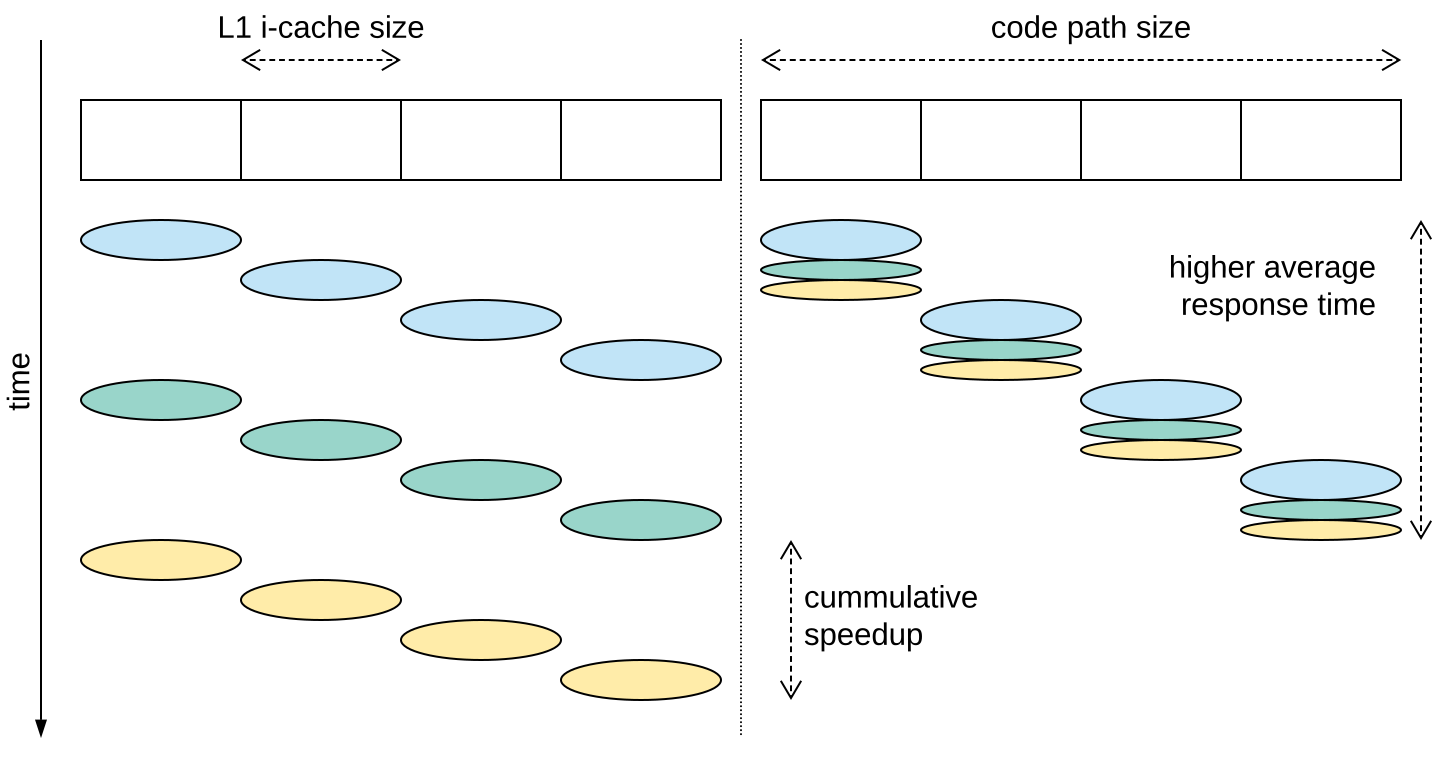
\includegraphics[width=0.8\textwidth]{fig_build/cohort_and_steps.pdf}
    \caption{
        Idealized scenario of three threads (different colors) executing the same code path that does not fit into the L1 cache.
        \textbf{Left}: each thread passes through the code completely before yielding CPU to the next thread.
        \textbf{Right}: team of threads trickles down the code path in code segments that do not exceed the L1 i-cache size.
    }
    \label{fig:cohort_and_steps}
\end{figure}

Blocking threads or threads aborting the transaction, would fall behind in this trickle-down schema and thus replace their ex-team members' cache state.
The solution is to remove threads aborting their transaction or blocking for synchronization and I/O from the team list and track them as \emph{stray threads}.
The publications on STEPS describe that the thread package in SHORE required modification to support this schema, but falls short on implementation details.
For this thesis, though, blocking is a highly relevant topic because it is a major problem in the proof of concept implementation at the KIT OS group (see Section~\ref{ch:relwork:kitpoc} and Chapter~\ref{ch:analysis}).
By examining the 6.0 release of SHORE which was published after STEPS, we can identify a base class for all DBMS threads called \texttt{sthread\_t} which provides wrappers for basic blocking I/O functions such as the \texttt{read} or \texttt{write} syscalls.
%Under the assumption that these abstractions existed in the version of SHORE that STEPS is based on, we can imagine that they were used to get notified about potentially blocking I/O requests by a thread in order to remove it from the team list.
%However, such an approach would not be able to differentiate between an actual block vs. non-blocking retrieval from the page cache and thus cause avoidable collateral damage to the thread requesting I/O.
%On the other hand, the code footprint of the I/O path could evict the team's working set from the cache --- an argument in favor of indistinguished removal from the team if I/O is pending.
Under the assumption that these abstractions existed in the version of SHORE that STEPS was based on, we are confident that the STEPS authors used these wrappers to get notified about potentially blocking I/O requests by a thread in order to remove it from its team list.~\cite{shoreRelease,shore}

Regardless of the exact implementation details, we are not convinced that the adoption of STEPS in arbitrary applications requires as few code modifications as claimed by the authors:
SHORE already comes with a custom thread abstraction around pthreads and centralized wrappers around blocking I/O.
In contrast, arbitrary applications will use the pthreads and C standard libraries directly, in which case
either substantial modifications to the code base are necessary to establish a situation as found in SHORE
or runtime-patching via \textsc{\texttt{ld\_preload}} would be required.

Lastly, STEPS's handling of stray threads should be considered: recall that stray threads are removed from their team when performing potentially blocking syscalls, and only re-join a team when being re-used for a new high-level operation.~\cite{steps}
Specifically, this means that STEPS does not account for the instruction footprint of the operating system at all.
However, \citeauthor*{osCacheFootprint} show that the operating system has a significant cache footprint and should thus be considered when trying to optimize the i-cache footprint.~\cite{osCacheFootprint,compspr} % osCacheFootprint: summary
Another perspective on the situation is that stray threads will continue to compete for CPU time for the time they are not blocked.
Since the OS scheduler is unaware of the team lists, it may schedule a stray thread in the midst of a team, evicting its cache state inadvertently.
STEPS tries to prevent this by giving a \textquote{hint} to the scheduler to prioritize the next thread that remained in the team, but does not elaborate on the additional syscall overhead.
By proposing a solution that is rooted in the OS's scheduler, we avoid the information loss and implementation complexities associated with STEPS's user-space approach.

\section{Top-Down Performance Analysis}\label{ch:relwork:topdown}
For the upcoming Section~\ref{ch:relwork:profiling} and the evaluation in Chapter~\ref{ch:eval}, we require some basic understanding of modern out-of-order processors and the top-down performance analysis method.

Modern high-performance microprocessors employ various techniques to exploit instruction-level parallelism (ILP) and to keep all functional units of the system busy.
\emph{Pipelining} is a very basic solution that splits the execution of an instruction into multiple phases. An instruction passes through an $N$-staged pipeline in $N * C_{max}$ clock cycles where $C_{max}$ is the number of clock cycles required for the slowest pipeline stage.
More sophisticated \emph{superscalar} processors replicate the functional units of individual stages, enabling multiple instructions to be completed (\emph{retired}) per clock cycle.
The dominant technique to manage this pipeline is called \emph{dynamic pipeline scheduling} where it is the job of the hardware instead of the software and compiler to optimally supply functional units with work.
Further techniques to exploit ILP are branch prediction and speculative execution.~\cite{hennessy2002DynamicPipeline}.

In any way, the above architecture is barely comparable to the classical model of a single-issue pipeline.
The terminology used in by Intel to describe their micro-architectures therfore refers to
an \emph{instruction fetch unit} that decodes the incoming instruction stream into micro-operations (uops),
an \emph{out-of-order execution engine} that executes those uops on functional units and
an \emph{in-order retirement} unit that ensures that the effects of the issued instructions appear in program order.~\cite{intelArchPipeline}.

\citeauthor{yasinTopdown}~\cite{yasinTopdown} further abstract this view by defining the
\emph{frontend} as the part of the CPU being responsible for fetching instructions, decoding them to uops and supplying them to the \emph{backend}.
The \emph{backend} in turn is in charge of fetching operands, scheduling uops on the functional units and retiring instructions in program-order.
The authors present the \textbf{top-down} performance anlysis method, which helps to identify micro-architectural bottlenecks by classifying CPU time into categories that are organized in a nested tree.
When applying the method, one traverses the tree top-down, usually following those categories marked with the highest percentage of spent CPU time.
The data source for the classification are performance counters which are built into to the CPU and are accessible by software.

For this thesis, we will focus on the \emph{top-level breakdown}, i.e., the highest level of the top-down hierarchy.
The categories at this level are \emph{Retiring}, \emph{Bad Speculation}, \emph{Backend-Bound} and  \emph{Frontend Bound}.
While the first two categories indicate that actually or at least potentially useful work was done, the latter two categories classify those pipeline slots lost due to microarchitectual bottlenecks:
Backend-bound cycles do not perform useful work because operations in the backend take exceptionally long, thereby introducing \emph{bubbles} into the execution pipeline.
Examples for this category may be a sub-optimal instruction mix or d-cache misses on uop-operands.
In contrast, frontend-bound cycles do not perform useful work because the backend is undersupplied with uops.
For example, i-cache misses will cause no instructions to be decoded and thus no uops to be issued for execution.~\cite{yasinTopdown,intelVtuneHelpRef,intelArchPipeline}

In this thesis, we optimize i-cache behavior by partitioning the instruction working set.
Reducing the percentage of frontend-bound cycles is thus used as a success metric.


\section{Profiling Datacenter Applications}\label{ch:relwork:profiling}
% alread shown that it's a problem in DBMSs, see 'affinity scheduling harizopoulos introduction' and the Steps paper (p3)
% dominant are the d-cache misses, but i-cache misses are also significantly higher than usual 
% growth of i-cache working set over time (speculation: due to product development) => worsens situation
% => stall cycles, X %
% memory latency, not band width

% TODO https://software.intel.com/en-us/vtune-amplifier-help-front-end-bound
While the micro-architectural performance problems caused by large i-cache footprints were already observed in \cite{cohort} and \cite{steps} in the early 2000s,
recent profiling work at Google shows that computer architecture is still not able to satisfy the requirements of contemporary scale-out applications.
However, the potential performance gains and cost savings due to improved cache behavior become relevant at scale, motivating a re-assessment of the situation.

\citeauthor*{kanev2015profiling} identify a significantly higher amount of pipeline stalls in real-world datacenter applications when compared to the SPEC CPU2006 benchmark.
Apart from the overhead associated with the distributed software architecture (RPC, serialization, etc) % datacenter tax
a large cache footprint (both code and data) reveals the major performance bottleneck on today's processors for typical datacenter applications:
the authors observe 60\% of $\mu$op slots to be backend-bound, and 15 -- 30\% to be frontend-bound, which leads to heavy under-utilization of the CPU cores' available resources at a micro-architectural level.\todo{do not require pre-existing knowledge about arch}
In particular, the authors find that more than 5\% of cycles are wasted due to empty front-end buffers, which is attributed to instruction read misses in the private L2 cache, resulting in slow accesses to the CPU's shared last level cache.
Additionally, the observations confirm that applications under active development grow in their instruction working set, worsening the situation.%
\footnote{The authors present exemplary results of up to 27\% per year.}
The authors do not explicitly investigate why datacenter applications have such large instruction working sets but mentioning \textquote{lukewarm} code and static linking as possible contributors.~\cite{kanev2015profiling}

In comparison to the work published a decade earlier (see Section~\ref{ch:relwork:cohort}~and~\ref{ch:relwork:steps}),
\citeauthor*{kanev2015profiling} focus on computer-architecture and only pay brief attention to the operating system:
approximately 20\% of CPU time is spent in the kernel with more than 5\% of CPU time in the scheduler alone.
Additionally, it is noteworthy that a 90-th percentile of the observed machines handles more than 4500 concurrent threads.
Given that at least a portion of these threads will be part of network servers, the question of the concurrency model thus stays very relevant although not explicitly stated as a source of performance-optimizations.~\cite{kanev2015profiling}

Looking at the related work presented so far, we conclude that for more than 15 years, typical datacenter applications have been observed to exhibit high i-cache-miss and branch-misprediction rates, resulting in sub-optimal use of the available CPU resources and motivting continued research in this field.

\section{Interim: Applicability to SMP Systems}\label{ch:relwork:anasmp}
Cohort scheduling, SEDA and STEPS were all evaluated on single-core machines.
Adaption to multi-core systems is not mentioned at all or stays theoretical.~\cite{steps,harizopoulos2003case}
Given today's ubiquitous multi-processors and the ongoing relevance of high i-cache footprints, re-examining the applicability of the above approaches seems appropriate.

\subsection{Private Caches}
% All numbers by example: My Haswell against STEPS CPU
% L1 and L2 are now oncore, L3 is shared (and inclusive on Intel)
% In contrast: early 2000s processors were single-core, L1 and L2
% capacities of L2 now what we have in L2 on-core
% today's L1 is split 32KiB i- and d-cache, early 2000s L1 64KiB (shared / unified?)  
% proof that today's chips are multicore: begin sodaspr
The single-core machines used to evaluate cohort scheduling, SEDA and STEPS feature a small L1 cache and a larger, higher-latency L2 cache.
However, contemporary symmetric multi-processors typically have a \emph{private} L1 and L2 caches and a \emph{shared} L3 cache.
The capacities of L1 and L2 are comparable to the early 2000s' models and the access latency between L1, L2 and L3 increases by a factor of 3 -- 4 between each level.
However, L2 instruction misses can typically not be compensated by out-of-order processing.~\cite{hennessy2002,haswellCacheLatency} %hennessy print page 509

An adaption of cohort scheduling and STEPS to multiprocessors must thus target the private caches of each core to achieve the similar benefits.
More importantly, the existence of private caches per hardware thread introduces the problem and opportunity to allocate this resource:
in terms of STEPS, multiple steps can now be spread over different cores instead of time-multiplexing the single available L1 i-cache.
We come back to this observation when assessing \emph{computation spreading} in Section~\ref{ch:relwork:compspr}.

\subsection{Real Parallelism}
We recall from Section~\ref{ch:relwork:cohort} that the scheduling trade-off in both approaches consists of reduced cache misses vs. increased response time due to \emph{batching}.
However, the real parallelism available on SMP systems brings with it another scheduling dimension that STEPS and cohort scheduling do not address:
to utilize the available hardware threads, load must be balanced among them to maximize resource utilization.
This goal surpasses response time since as the primary scheduling goal since the the service provider generally pays for the number of cores, not their actual usage.\todo{well actually... cpu time accounting}
All relevant operating systems abstract CPU cores through threads, and the OS scheduler implements load balancing by migrating threads between cores, often directed by metrics such as the length of each core's the ready queue (\emph{load}).~\cite{freeBSDSchedulerLoad}

Cohort scheduling and STEPS were not designed for this situation because
%both solutions include \emph{batching} as a central element, either at the syscall boundary or at arbitrary points in the application code (see Section~\ref{ch:relwork:cohort}~and~\ref{ch:relwork:steps}).
\textbf{batching is inherently not work-conserving on SMP systems}:
all threads in a cohort or team must run on the same core in order to benefit from the warm i-cache, but this means only one thread per team can run at any given time.
Furthermore, STEPS and the OS scheduler work actively against each other because the latter will see all threads in a cohort as runnable and actively spread the cohort over all (presumably idle) cores,
destroying all promised performance benefits.

An easy fix would be a mechanism for STEPS to influence the load balancing in order to favor threads of the same team to stay on the same core, e.g., through thread pinning.
This is obviously not work-conserving on multi-core systems, requiring additional mechanisms and communication between STEPS and the OS to fix it.
On a busy system, one could also argue that enough threads are available to simply employ cohort-scheduling per core.
However, in contrast to the approach of \emph{computation spreading} presented in the next section, this replicates to each core the repeated capacity misses when a team moves to the next step.

The above assessment shows that cohort scheduling, SEDA and STEPS cannot be directly applied to today's multi-processor systems.
The availability of private caches per core must be accounted for and new requirements such as load balancing between cores must be addressed.
However, given the ongoing relevance of the problems identified more than 15 years ago, we continue this chapter by investigating publications that explicitly target multi-processor systems.
\todo{s/multi-processor/multi-core/?}

\section{Computation Spreading}\label{ch:relwork:compspr}
% TODO: related and actually more relevant to our approach: Computation Spreading
% => term: destructive interference
% => migration for syscall => split i-working set (naturally) + little communication (because sendfile)
\emph{Computation spreading} (CSP) in its most general form is a technique to cache the instruction working set of a process more effectively on SMP systems which commonly feature private caches per core.
\citeauthor*{compspr} show that this cache hierarchy leads to redundantly stored code.
For example, in a traditional thread-based concurrency model, each request-handling thread may interact with the file system through system calls which leads to redundantly stored file system code being in each core's private cache.
The authors present a solution that temporarily assigns CPU cores to either execute OS code or user-level code, exploring and evaluating several allocation policies.
Threads entering or leaving the OS synchronously through syscalls, exceptions or page faults are then migrated between compatible cores.~\cite{compspr}

A central aspect of the implementatio is the thread migration mechanism which is based on hardware virtualization features:
all synchronous kernel entries are intercepted and used to trigger the thread migration, leaving the \textit{guest} OS and user-space software completely unmodified.~\cite{compspr}
An easy-to-overlook detail however is that the hardware-based thread migration is only available in hypervisor mode, which means that cooperation from the software executing in this mode is required.
Deployment in public clouds based on hardware-virtualization is thus only possible with explicit support by the cloud provider and would thus require further work in the hypervisor scheduler.
Our solution does require hardware virtualization due to limited driver support but implements thread migration in software and can thus be deployed to existing infrastructure.

The authors evaluate their solution using full-system simulation of an eight-core machine with private L1 and L2 cache and a shared L3 cache.
Server applications, which are of primary interest for this thesis, exhibit 25 -- 58\% fewer L2 instruction misses and 9 -- 25\% improved branch misprediction rates.
Data read misses are less affected, with only 13 -- 19\% decrease for Apache web server and an OLTP application.
The approach leads to a speed-up of up to 20\% in Apache and 9.4\% in OLTP measured by the total runtime of the full-system simulation.~\cite{compspr}

Despite the very specific implementation, it should be noted that the concept presented by the authors is more general and not limited to the syscall interface:
they suggest migration points at arbitrary positions in the application code and corresponding core allocation policies.~\cite{compspr}
However, we cannot find a proposal to implement this, which is a very welcome segue to the next section.
\todo{hardware-based approaches?} % http://ieeexplore.ieee.org/document/1410076/

\section{Prototype in Linux at the KIT OS Group}\label{ch:relwork:kitpoc}
%TODO this section should coin the term stage-aware scheduling, otherwise, we need to do that before the analysis --- rename section with stage-aware in title
\NewDocumentCommand{\klt}{}{\textsc{klt}\xspace}
\NewDocumentCommand{\klts}{}{\textsc{klt}s\xspace}
\NewDocumentCommand{\ult}{}{\textsc{ult}\xspace}
\NewDocumentCommand{\ults}{}{\textsc{ult}s\xspace}
A Linux-based proof-of-concept implementation at the KIT OS group combines the idea of staged execution, cohort scheduling and computation spreading into a C API that allows for intuitive conversion of existing code bases to staged execution:
the application developer manually identifies stages and inserts library calls into application code for switching the current stage.
Each CPU core is assigned one or more stages and each time a thread switches to a new stage, it is migrated to a core assigned to that stage, benefiting from a warm i-cache.
Obviously, this approach targets applications that employ thread-based concurrency, i.e. the multi-threaded server architecture outline in Section~\ref{ch:relwork:concmod}, since the stage-switching is embedded into the control flow of the request handler and thus not explicitly modeled like in SEDA (see Section~\ref{ch:relwork:seda}).

Fast thread migration mechanism is required for this technique to succeed
--- otherwise, the performance benefits of always-warm caches per stage are destroyed by the migration time.
%\newcommand{\setaffinity}{\texttt{sched\_setaffinity(2)}}
The Linux built-in facility for this purpose, \texttt{sched\_setaffinity}, is impractical because it uses
expensive inter-processor-interrupts to implement this syscall, resulting in $9\mu s$ -- $14\mu s$ of migration time.
As a consequence, thread migration was implemented in user-space:
for each user-level thread (\ult), there still exists exists a kernel-level thread (\klt),
but \klts are pinned once to a specific core and stage.
\ults run on a \klt of the stage they are currently in and migrate to a different \klt when switching stages.~\cite{sodaspr}% sodaspr:table 1

When a \ult makes a call to switch stages, its context is saved and enqueued into the next stage's incoming migrations queue.
The originating \klt now waits for new \ults on its own stage's incoming migrations queue.
If it is empty, the \klt makes a blocking syscall \texttt{sys\_dequeue} to a kernel component to wait for incoming migrations.
The kernel component must ensure that there is always one \klt per core either doing work or actively dequeuing \ults in order to utilize the CPU.
This is implemented by a callback from the Linux scheduler that informs the kernel component of task state changes.
For example, if the currently dequeuing \klt $K_1$ executes a \ult, and that \ult blocks on a mutex, $K_1$ transitions from \texttt{running} to \texttt{blocked}.
The kernel component must wake up another \klt $K_2$ that is currently waiting for incoming migrations of that stage on that core.
Otherwise, the core does not perform any work (for the application) until $K_1$ acquires the mutex and becomes \texttt{runnable}.
Figure~\ref{fig:kit_os_poc_blocking} visualizes this situation.

\begin{figure}[h]
    \centering
    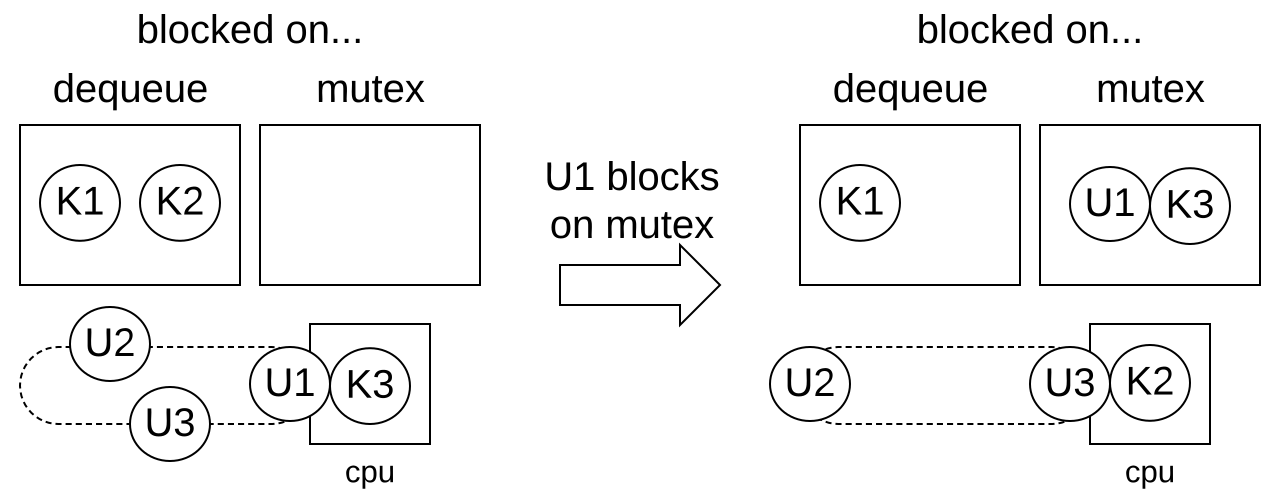
\includegraphics[width=0.8\textwidth]{fig_build/kit_os_poc_blocking.pdf}
    \caption{When a \ult issues a blocking syscall, the current \klt blocks. Another \klt must take over executing \ults from the core's queue. Note that while there is a \klt for each \ult, the relationship is not fixed.}
    \label{fig:kit_os_poc_blocking}
\end{figure}

The authors evaluate their design with microbenchmarks and performance-counters, showing x\% fewer i-cache misses, y\% fewer mispredicted branches.
Additionally, a full-system evaluation is made by comparing the benchmark results of the TPC-C OLTP benchmark on Linux 4.X between an upstream and a \emph{stagified} version of MySQL 5.6.38 running on an SMP system with X cores.
The expected reductions of i-cache and mispredicted branches are achieved in the stagified version, but overall throughput depends on the number of concurrent requests.
taking upstream as baseline (100\%), throughput with a single TPC-C terminal is z\% higher in the stagified version, but multiple terminals and thus concurrent requests leads to Z2\% of upstream's throughput.
The proof-of-concept is thus clearly not work-conserving on SMP systems, which we will investigate in the next chapter.
\todo{data}

\chapter{Analysis}\label{ch:analysis}
Related work has demonstrated that spreading the working set of an application over multiple cores yields lower on-core cache miss rates.
The proof-of-concept implementation at the KIT OS group furthermore shows that large-scale refactoring of existing code bases is not necessarily required to spread the working set:
given an application with a suitable threading model, patches of a few lines are sufficient to reduce i-cache misses and branch-misprediction significantly.

However, its evaluation on an SMP system shows that the solution is not work-conserving as visualized in Figure \ref{fig:kit_os_poc_work_conserving}:
imagine a system with multiple cores per stage and a \ult $U_1$ in stage $S$ executing on a \klt $K_1$.
As described above, $K_1$ is pinned to core $C_1$.
When $U_1$ performs a blocking syscall, for example when trying to acquire a lock, $K_1$ blocks.
The Linux scheduler now dispatches another task $T$ on $C_1$ to maximize CPU utilization, where $T$ is not a $K_i$ of our application.
In fact, all $K_i$ are blocked in \texttt{sys\_dequeue}.
When $K_1$ finally acquires the mutex and is \texttt{ready} again, it is still pinned to $C_1$ because the solution needs this to perform thread migration in user-space.
However, $C_1$ is still executing $T$, not $K_1$, and thus $K_1$ must be put into $C_1$'s ready queue.

The problem at this point is that there may exist \emph{another} CPU $C_2$ where a \klt $K_2$ is dequeuing \ults in the \emph{same stage} $S$:
if $K_2$ does not have any \ults to execute, $K_1$ should be migrated to $C_2$ immediately when it is woken up and continue execution there, benefiting from the warm on-core caches.
But the implementation only performs thread migration when a \ult calls the stage switching API.
There is no mechanism in place to save $K_1$'s state and enqueue it to $K_2$'s incoming migration queue on wake-up.
One might assume it is possible to enqueue $U_1$ to $K_2$ since we saved its register state on kernel entry via \texttt{pthread\_mutex\_lock}:
this is not possible because there might still be kernel code that needs to run after the mutex is acquired, before returning to $U_1$.

\begin{figure}[h]
    \centering
    
\includegraphics[width=0.8\textwidth]{fig_build/kit_os_poc_work_conserving.pdf}
    \caption{The proof-of-concept implementation is not work-conserving. When K1 becomes ready it should be dispatched to C2 immediately. But K1 is pinned to C1 due to the implementation of thread migration.}
    \label{fig:kit_os_poc_work_conserving}
\end{figure}

We identify several fundamental problems in the approach taken by the proof-of-concept implementation:
the requirement for fast thread migration drove the design toward a user-space solution which decouples the threads known by the application (\ults) from the threads known by the kernel (\klts).
However, the kernel scheduler still only handles \klts and assumes a 1:1 threading model, which leads to an \textbf{ambiguous role of \klts} in the proof-of-concept:
when switching between stages, the user space thread migration code views \klts as the CPUs they are pinned to.
But when a \ult running on a KLT interacts with the Linux kernel, the kernel sees a normal \texttt{task\_struct} and continues to assume the 1:1 threading model where tasks can just block.
The proof-of-concept works around this schizophreny by introducing a callback from the scheduler to react to blocking \klts, but fails to handle asynchronous events like wake-ups.
The latter leads to non-work-conserving behavior on multi-core systems.

We conclude that the proof-of-concept does not model the situation correctly: the association of stages and CPU cores is piggybacked onto the \klts using \texttt{sched\_setaffinity}, leading to an ambigous role of \klts.
We thus propose that stages must be modeled explicitly in the kernel and be separate entities, beneath CPUs and threads:
\begin{itemize}%
    \item The association of stages and CPU cores must be represented explicitly.
    \item Threads must carry the information in which stage they are executing.
    \item The scheduler must honor this information by scheduling threads onto cores that are associated with their respective stage.
    \item The scheduler must trade off the potential gains of always-warm caches against existing scheduling goals such as resource utilization, fairness and response time.
\end{itemize}%
This reverts the complex situation of \ults and \klts to a simple 1:1 threading model, removing the special-case of blocking kernel activity.

The remainder of this thesis presents our design as well as its implementation in the OSv library operating system and the evaluation using microbenchmarks and the TPC-C benchmark with MySQL.\todo{repetitive?}

\chapter{Design \& Implementation}\label{ch:di}
Certain classes of datacenter applications exhibit large instruction working sets that do not fit into the private cache of commodity processors.
On a micro-architectural level, this leads to underutilization of the cores' available computing resources, and thus worse application performance.
This chapter presents our operating-system-based solution to mitigate this problem in multi-threaded servers.

Multi-threaded servers handle client connections in threads, each following the same, sequential, potentially blocking, code path.
For example, in a database management system that is accessed over TCP, a request-handling thread will
\begin{enumerate}[label=(\alph*)]
    \item read the request data from a socket, using the network stack, \label{en:di:ov:read}
    \item deserialize \& parse it, \label{en:di:ov:des}
    \item perform the requested operation,\label{en:di:ov:processing}
    \item serialize the response and \label{en:di:ov:ser}
    \item send it back to  the client. \label{en:di:ov:write}
\end{enumerate}
While not true for all types of servers, database systems for example exhibit a a significant i-cache footprint in step~\ref{en:di:ov:processing} per high-level SQL operation (see Section~\ref{ch:relwork:steps}).
The code footprint of the network stack is also significant, as is the filesystem and potentially the serialization library.

All these steps together will execute more code than fits in the private i-cache, leading to capacity i-cache misses when executed on a single core.
Additionally, some code will be executed twice, but with another i-cache sized working set inbetween:
For example, steps \ref{en:di:ov:read} and \ref{en:di:ov:write} share parts of the network stack but have steps \ref{en:di:ov:des}, \ref{en:di:ov:processing} and \ref{en:di:ov:ser} inbetween.
Step \ref{en:di:ov:write} will thus likely incur i-cache misses for code that step \ref{en:di:ov:read} had brought into the cache at the beginning of the procedure.
Furthermore, we must consider the situation where a request-handler thread $A$ blocks, for example on I/O in steps \ref{en:di:ov:read}, \ref{en:di:ov:processing} or \ref{en:di:ov:write}:
The scheduler will dispatch another request-handler $B$ on the same core, which may be in a different step than $A$.
At worst, $B$ will evict all of $A$'s cache state.
Looking at multi-core systems, the above behavior can be observed on each core because contemporary OS's schedulers balances threads based on load of the cores, not on cache state.

We solve above problems on modern multi-core systems by implementing a suitable scheduling policy in the OS scheduler.
\textbf{We define a \emph{stage} as a span in the request-handling code path that has an instruction working set smaller than the private i-cache size.}
Ideally, different stages' instruction and data working sets are fully disjoint.
Given the example database system, one would define the following stages:
$S_n$ for network stack, $S_{ser}$ for serialization and one per SQL operation ($S_{INS}$ for \texttt{\textsc{insert}}, $S_{SEL}$ for \texttt{\textsc{select}}, \dots).
It is important to emphasize that stages do not necessarily form a pipeline:
Reading from and writing to the network socket form one stage because these operations share the network stack code, as do request deserialization and response serialization because they both use the serialization library.
\todo{well actually, ser and des may be quite disjoint, but it still works...}

Once the stages are defined, a request-handler thread must switch to the appropriate stage before performing the next step of request-handling.
In concrete terms, this means that developers must call a system API in the request-handling code path.
In the example above, a \textit{\textsc{select}} request would result in the following switch series: $S_n$, $S_{ser}$, $S_{INS}$, $S_{ser}$, $S_n$.

%%From an application developer's perspective, we provide a system API allowing to define \emph{stages} on program start and switch a thread as objects and to switch the current thread between them.
%%Stages represent ideally disjoint instruction working sets, each fitting into the private cache of a CPU core.
%%The application developer \emph{stagifies} their application by inserting stage switching calls into the request-handling code path, thus partitioning its total instruction working set into stages.
%%
%%In the above example, one would thus define stages for interaction with the network stack, for serialization and each SQL operation, i.e., \texttt{INSERT}, \texttt{SELECT}, etc.
%%Before calling \texttt{read} or \texttt{write} on the network socket, the developer would then switch to the network-stack-stage.

Given such a \emph{stagified} application, we then track per thread the association to its current stage in the TCB and per stage the number of threads runnable threads currently associated with it.
We use this information to periodially compute the \emph{current core allocation}, which assigns CPU cores to stages proportional to the stages' load.
A core is thus always allocated to exactly one stage. % however, a stage may not have any dedicated cores. only tell that in the details section
The scheduler then implements the following guiding principle: \textbf{A thread is only dispatched on cores that are allocated to the thread's current stage}.
When a thread uses the system API to switch to a stage $S$, we choose the least-loaded core $C$ among the cores allocated to $S$ and enqueue the switching thread into $C$'s runqueue.
When a thread blocks, it no longer counts toward the load of stage but does not lose the association to it.
Thus, when a blocked thread is woken up again, the \emph{waker} simply uses the current core allocation to choose a suitable core for the woken thread and enqueue the still-sleeping thread into that core's runqueue.

\begin{figure}[h]
    \missingfigure{visualize the solution}
    \caption{TODO}
\end{figure}

The promise behind this approach is the same as in computation spreading and the proof-of-concept implementation at the KIT OS group (Chapter~\ref{ch:relwork}):
\textbf{By dedicating CPU cores and hence their private caches to a stage and by scheduling threads exclusively on the cores of their current stages, the i-cache always contains the instruction working set of all threads in the CPU's runqueue.}
This reduces instruction cache misses, pipeline stalls and mispredicted branches, resulting in faster execution of the stage's code and cheaper context switches on the CPU. \todo{an argument for preemptive round robin}

Our solution is specific to certain types of server applications and thus not suitable as a general-purpose scheduling policy.
Ideally, we would thus extend an existing scheduler such as the Linux CFS.
However, this is out of scope of this thesis due to the expected design and implementation complexity.
Instead, we implement our solution in the OSv library operating system, a small kernel that is bundled with an application into an appliance-like virtual machine image.

The remainder of this chapter presents our design and its implementation in detail:
Section~\ref{ch:di:osv} gives an introduction to the OSv library operating system, providing the knowledge required to understand the implementation constraints we faced.
We proceed with details on the user-space API illustrated with examples (Section~\ref{ch:di:api}), followed by the design of our thread migration mechanism (Section~\ref{ch:di:mig}).
In Section~\ref{ch:di:wake}, we explain the details involving the wake-up mechanism which required significant re-working of OSv's thread state tracking.
Section~\ref{ch:di:pol} then presents the CPU core allocation policy.
We conclude with a discussion of the limitations and trade-offs of our design in Section~\ref{ch:di:discuss}.
Where appropriate, we refer to the relevant commits in the Git repository of our modified version of OSv.

\section{The OSv Library Operating System}\label{ch:di:osv}
We implement our stage-aware scheduling solution in the OSv \emph{library operating system}, which rethinks the traditional divide between the kernel and applications:
Traditionally, an operating system provides abstracts from the physical hardware and multiplexes it among \emph{multiple} untrusting users and applications, providing protection and isolation at various levels.
With the rise of hardware virtualization, it has become common practice to deploy a traditional OS running a \emph{single} application in a virtual machine running on top of a hypervisor.
In this situation, both the hypervisor and the guest kernel implement protection mechanisms, but because each VM only runs a single application, the protection efforts of the guest kernel may be considered duplicate.~\cite{mirageOS,osvMain}

OSv addresses this situation by delegating all resource abstraction and protection responsibilities to the hypervisor.
It confines itself to providing a familiar execution environment for a \emph{single trust domain}, providing facilities for multi-threading, scheduling, a network stack and filesystems.
To run an application on OSv, it is bundled with the OSv kernel into a virtual machine image.
When the VM starts, OSv establishes a \emph{single virtual address space} and dynamically links the application against its own C standard library, in which system calls are merely function calls into OSv routines.
This technique allows dyanmically linked applications built on Linux to execute unmodified on OSv, unless they depend on facilities intentionally not provided by OSv such as forking new processes.
The single trust domain property furthermore allows omitting all privilege level switching between OSv and the application.
In summary, the removed user-kernel-boundary, syscall overhead and context \& privilege level switching improves application performance significantly without any application code changes required.
However, if application developers choose to specifically target OSv, more efficient system APIs provide further optimization, e.g. zero-copy networking as opposed to the traditional socket API.~\cite{osvMain}

While OSv incorporates pre-existing components for ACPI, the filesystem and originally the network stack, the core system is implemented in C++11.
The codebase of ca. $400000$~lines of code is very small compared to the 20~million lines of Linux 4.13, % both code and comments
% Linux: cloc . (v4.13)
% OSv: cloc core include bsd arch fs drivers scripts linux.cc runtime.cc loader.cc Makefile (v0.24-470-gf9eedad4)
which can be attributed to both the use of a more expressive programming language and the comfort of only providing device drivers for typical hypervisor-emulated devices and paravirtualization.
The OSv scheduler in particular amounts to less than 3000 lines, making OSv particularly attractive for this thesis.%cloc core/sched.cc include/osv/sched.hh
~\cite{osvMain}

\subsection{The OSv Scheduler}\label{ch:di:osv:sched}
The solution presented in this chapter must be implemented in the scheduler.
To understand the design and implementation constraints we faced, this section gives a summary of the upstream OSv scheduler implementation.

The OSv developers state that the \textquote{thread scheduler [\dots] should be lock-free, preemptive, tick-less, fair, scalable and efficient.}
As such, it features CPU-local runqueues containing runnable threads, which are sorted ascendingly by the threads' recent average rumtimes.
Load-balancing is implemented by a periodically-invoked per-core load-balancer thread that migrates threads from its runqueue to other cores if these are less loaded.~\cite{osvMain}

OSv implements thread migration through a set of lock-free single-producer-single-consumer queues:
Given $N$ CPUs, each CPU has $N$ \texttt{incoming\_wakeup} queues, one per source CPU, containing pointers to the TCBs of the threads being migrated.
At every reschedule, a CPU then drains all incoming queues into its runqueue.
Each CPU is guaranteed to have an always runnable idle thread that spins for a short time and HALTs the CPU if no other runnable threads are in the runqueue.
Thus, a source CPU may need to send an inter-processor-interrupt (IPIs) to the target CPU after enqueuing the migrated thread.
For this purpose, each CPU has a bitmask, each bit representing one source CPU / wakup queue:
The source CPU will atomically set its bit in the target CPU's bitmask and only send the IPI if the bit was not set before.
This avoids flooding the target CPU with IPIs from different cores.~\cite{osvGit,osvMain}
\todo{mention that they could use mwait here? we need that in the evaluation}

Migrating runnable, but not currently running threads, is easy in this model:
the source CPU removes the runnable thread from its runqueue and puts it into the incoming queue of the target CPU.
However, threads may also migrate themselves to another CPU while still running, for example through the \lstinline[style=figurecpp]{pthread_set_affinity} API.
Let us call this case \emph{synchronous thread migration}:
In OSv, the migrating thread spawns a short-lived helper thread and immediately schedules out.
The helper thread will then put the migrating thread's TCB into the correct \lstinline[style=figurecpp]{incoming_wakeup} queue.~\cite{osvGit}

One complication of the above procedure are timers:
Apart from timers specific to a CPU, a thread can program timers as well, for example for use with \textsc{\texttt{sigalarm}}.
Per CPU, a list of active timers is kept, sorted ascendingly by their expiration time.
The OSv timer implementation then programs a signle hardware-timer (\lstinline[style=figurecpp]{clock_event} driver) such that it fires at the nearest expiration time.
On x86-64, the CPU-local Advanced Programmable Interrupt Controller (LAPIC) timer is used for this purpose.~\cite{intelSDMLAPICTimer}
In the timer interrupt handler, the expired timers are removed from the sorted list and the LAPIC timer is reprogrammed.
Threads whose timer fired are then woken, i.e., marked as runnable and put into the CPU's ready queue.
It is crucial to observe that the upstream OSv timer abstraction does not allow a thread to have timers set on multiple CPUs:
All data structures related to timer management are only protected by masking interrupts because they are only manipulated by the thread itself or from the timer interrupt context.
For thread migration, this means that timers must be removed from the source CPU's timer list before enqueuing the thread into the target CPU's \lstinline[style=figurecpp]{incoming_wakeup} queue.
On the target CPU, after adding the migrated timers to its timer list, the LAPIC may need to be reprogrammed if any of the migrated timers' expiration dates are earlier than the previous head of the list.~\cite{osvGit}

In addition to synchronous thread migration upstream OSv also supports \emph{remote asynchronous thread migration}, i.e., the situation where a thread $T_i$ executing on CPU $C_1$ initiates the migration of a thread $T_m$ currently executing on a CPU $C_2$ to a CPU $C_3$.
As outlined in the previous paragraph, $T_m$'s timers must be migrated, which can only be initiated from the source CPU itself.
Upstream OSv only requires this feature for implementing \lstinline[style=figurecpp]{pthread_attr_setaffinity_np} and uses a helper thread $T_h$ that chases $T_m$ until $T_h$ can successfuly mask all interrupts on the same CPU as $T_m$ and suspend $T_i$'s timers.
The remaining steps are the same as in synchronous thread migration.~\cite{osvGit}


\section{The Stage API}\label{ch:di:api}
% User-space can enqueue itself to a stage, will be migrated to one of the cores it is assigned to
% Stack structure for implementation comfort, describe idea behind stack structure & guards -> spans, like in web browser
Our scheduling policy spreads an application's working set over the private caches of all available CPU cores by scheduling threads only on those cores that have its current stage's code in their private cache.
We require developers to manually \emph{stagify} their applications by defining stages and inserting switching calls into the request-handling code path.
In order to facilitate adoption, our primary design goal for the stage API is thus to be non-invasive, allowing maintenance of private patches to an existing open source code base.

In OSv, we implement stages as a C++ class with public member functions for stage definition and switching.
Since kernel and application share a single trust domain, we can simply export the same header to applications.
A stagified application will thus receive pointers to the kernel objects representing changes and invoke methods on them.
However, applications for OSv must be built on the Linux host where the stage API header and implementation is not available.
To avoid build and linker failures, we provide a no-op implementation of the API as a shared library, enabling us to produce application binaries that work on both Linux and OSv.%
\footnote{The OSv linker ignores missing libraries, and the app does not crash because the OSv implementation of the stage class provides the required functions.}
Figure \ref{fig:di:api:exampleraw} gives an impression of how the stage API could be used in an existing application.

\begin{figure}
\begin{lstlisting}[style=figurecpp,morekeywords={stage,stage::define,enqueue}]
#include <osv/stagesched.h>

stage *s_net, *s_ser, *s_db;

int main() {
  s_net = stage::define("net");
  s_ser = stage::define("serialization");
  s_db = stage::define("db");
  // start threads ...
}

void request_handler(database db, net::conn c) {
  s_net->enqueue();
  buf b = c.recv();
  s_ser->enqueue();
  req req = sql::parse(b);
  s_db->enqueue();
  response resp = db.handle_request(req);
  s_ser->enqueue();
  buf b = sql::respond(resp);
  s_net->enqueue();
  c.send(b);
}
\end{lstlisting}
\caption{Example for a stagified application using the stage API in pseudo C++. Because we implement our solution in OSv, we can simply use pointers to the kernel objects representing stages.}
\label{fig:di:api:exampleraw}
\end{figure}

In addition to the direct invocation of the switching API, we provide a RAII-style data-structure reminiscent of C++11 lock guards to switch to a stage for the lifetime of a block and switch back to the previous stage when the guard object goes out of scope.
This can be used to shift the responsibility of switching stages from the function caller to the callee, which is particularly useful when a piece of code is large enough to have its own stage but is called from more than one other stage.
Figure~\ref{fig:di:api:examplestack} shows how the above example looks like with the RAII-style API.

\begin{figure}
\begin{lstlisting}[style=figurecpp,morekeywords={stage_stack,stage,stage::define,stage_stack::guard}]
#include <osv/stagesched.h>

class thread {
    stage_stack stagestack;
    ...
};

stage *s_net, *s_ser, *s_db;

int main() {
  s_net = stage::define("net");
  s_ser = stage::define("serialization");
  s_db = stage::define("db");
  // start threads ...
}

void thread::request_handler(database db, net::conn c) {
  buf b = c.recv();
  req rq = sql::parse(b);
  response rs = db.handle_request(rq);
  buf b = sql::respond(rs);
  c.send(b);
}

// Use stage_stack::guard in all functions
req sql::parse(buf& b) {
  stage_stack::guard g(thread::current()->stagestack, s_ser);
  ...
}

\end{lstlisting}
\caption{\lstinline[style=figurecpp]{stage_stack} keeps previous stages in a stack.
    The \lstinline[style=figurecpp]{stage_stack::guard} constructor pushes the stage pointer onto the \lstinline[style=figurecpp]{stage_stack} and switches to the stage.
    The corresponding destrucutor pops the current stage's pointer from the stack and switches back to the previous stage.}
\label{fig:di:api:examplestack}
\end{figure}

The commits in the Git repository corresponding to the changes presented in this section are \refosvcommit{439b55014ea8d3285db7523c4c1ba02b4948cd41} and \refosvcommit{9eaf3a8b9aa5a18a5a79920066803a5a84d3b6c5}.

\section{Fast Thread Migration}\label{ch:di:mig}
% Motivation: Stage switch requires migration to other core
% Existing migration mechanism is based on IPIs, is too slow => results, maybe also compare to Linux => adjust hopper
% Must be fast, because of opportunity cost calculation:
%   -> for single client:       cold cache and no migration vs warm cache but migration times
%   -> for T > #cpus clients: ???
% Design:
%       stage migration and hence migration to other CPU core is synchronous to program flow
%       MPSC queue per CPU, for incoming stage migrations
%       on stage switch, evaluate CPU allocation policy, pick target CPU, enqueue into stagesched_incoming
%       target CPU dequeues from stagesched_incoming in idle thread -> mention potential optimization: mwait
%       Measurement results: why not here??? specifically if we discuss mwait?
% Implementation:
%       a stage switch means scheduling out on the source CPU, being migrated to the target CPU and resuming execution there
%       per-cpu MPSC queue that contains pointers to TCBs of threads in stage migration
%       cpu idle thread dequeues from mpsc
%       additional thread states for thread in stage migration
%       critical race condition:  only after scheduling out on the source CPU must execution continue on the target CPU,
%           but thread puts itself into the MPSC queue while it is still executing
%           => augment the thread-switching routine (which is the last code the migrating thread execute on the source CPU) to atomically
%              switch the state of the thread from stagemig_run to stagemig_sto
%           => target CPU only dequeues those threads that are in stagemig_sto to its runqueue, others are still executing code on the source CPU
% => State diagram with changes made in this step
Once an application has been stagified by the application developer, our solution must act on the stage switching calls made during request handling.
Specifically, we must find a core whose private caches contain the next stage's code and migrate the calling thread to that core.
We defer discussion of the core allocation policy to Section~\ref{ch:di:pol} and focus on the migration mechanism for now.

For a net benefit from spreading the instruction working set, the performance gained through always warm i-caches must outweigh the cost of thread migration.
One signficant contributor to the latter is migration latency, which is the reason why we require a low-latency mechanism.
Upstream OSv's uses short-lived helper-threads for synchronous thread migration and inter-processor interrupts (IPIs) to notify the target CPU about incoming migrations.
The IPIs are necessary because the target CPU may be temporarily \textsc{\texttt{halt}}ed in the idle thread.
\textbf{We state that upstream mechanism is unsuitable for our use-case of frequent stage-switching:}
At first, recent measurements on AMD systems have shown that IPI propagation on bare-metal systems is ~1700 ns~\cite{ipiLatencyPopcornLinux}. % (2,2Ghz machine, 7501 Round-Trip-Time, sec 6.2.2) (7501×1000000÷2200000000)÷2
For OSv, we assume significant overhead due to virtualization, which we will further investigate in Section~\ref{ch:eval:mig}.
The IPI propagation time puts a lower bound on the achievable migration latency but additionally, the impact of IPIs on the target CPU's pipeline must be considered:
An arriving interrupt will flush the pipeline or at least obsolete the instructions it currently executes. \todo{proof? found on stackoverflow} %https://stackoverflow.com/questions/8902132/when-an-interrupt-occurs-what-happens-to-instructions-in-the-pipeline
% cache pollution in OSv is insignificant because the IPI literally does nothing
Lastly, on the source CPU, the use of helper threads implies memory allocation for the new TCB and an invocation of the OSv scheduler, which does not run in constant time.

\textbf{As a consequence of the above, we choose to implement a lower-latency alternative for thread migration that neither uses IPIs nor helper threads}:
When a thread switches to another stage, the switching thread queries the core allocation policy for a target CPU that has the target stage's code in its private caches.
The thread then puts its TCB into the \emph{incoming migrations queue} of the target CPU \emph{while running} and subsequently schedules out.
The target CPU's \lstinline{reschedule} routine and its idle thread eventually dequeue the TCB pointer from the incoming migrations queue into the runqueue, thereby completing the migration.

While the above paragraph gives a good overview of our mechanism, we omitted two important details:
At first, there is a race condition between the point where a migrating thread $T$ puts its TCB pointer into the incoming migrations queue and the point at which it schedules out: \todo{refer to steps in the figure}
If the target CPU dequeues $T$'s TCB before $T$ has scheduled out, the TCB contains will invalid register state or the state from the last time $T$ scheduled out.
If $T$ now starts running on the target CPU, we have the hazardous situation of $T$ running on both CPUs simultaneously, primarily visible through a corrupted stack.
We solve this problem by representing the stage-switch as a \emph{two-step} thread state transition:
Before the migrating thread puts its TCB into the target CPU's incoming migrations queue, it sets its state to \lstinline[style=figurecpp]{stagemig_run}.
The target CPU will not put threads in that state into its runqueue but instead enqueue it back into the incoming migrations queue because the migration is not yet finished.
On the source CPU, after $T$ has scheduled out, we then set $T$'s state to \lstinline[style=figurecpp]{stagemig_sto}.
Eventually, the target CPU will dequeue $T$ again, observe from its state that it is not running anymore and enqueue it into its runqueue.
The procedure described above is visualized and Figure~\ref{fig:di:mig}.

\begin{figure}
    \centering
    \subcaptionbox{T is running on core2 and wants to migrate to core1.}[6cm]{
    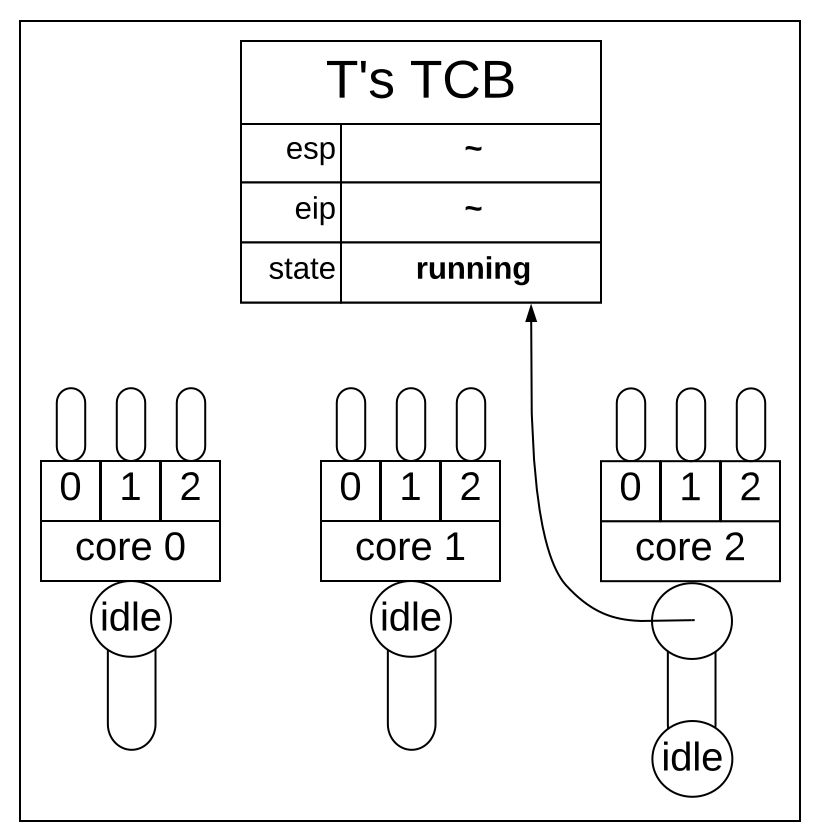
\includegraphics[width=5cm]{fig_build/mig0}
    }
    \hspace{1.2cm}
    \subcaptionbox{T switches to \lstinline[style=figurecpp]{stagemig_run} and puts a pointer to its TCB into the incoming migrations queue at core1.
        Core1's idle thread does not dequeue TCBs with state $\ne$ \lstinline[style=figurecpp]{stagemig_sto}.}[6cm]{
    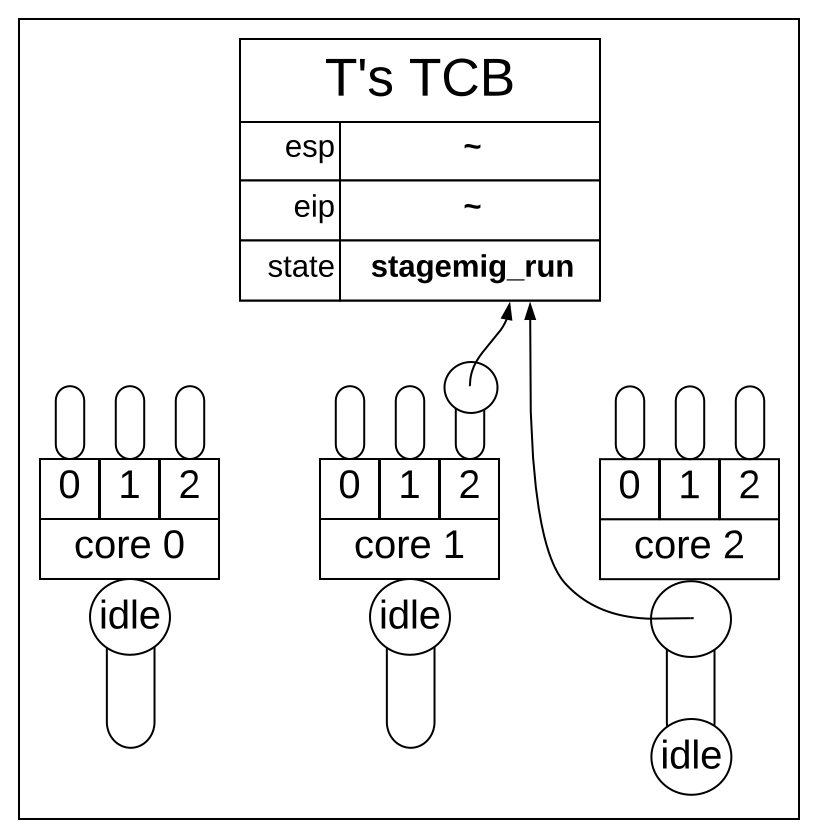
\includegraphics[width=5cm]{fig_build/mig1}
    }
    \hfill
    \par
    \bigskip
    \subcaptionbox{T schedules out. The context switching routine sets its state to \lstinline[style=figurecpp]{stagemig_sto} after T has stopped running on core2.}[6cm]{
    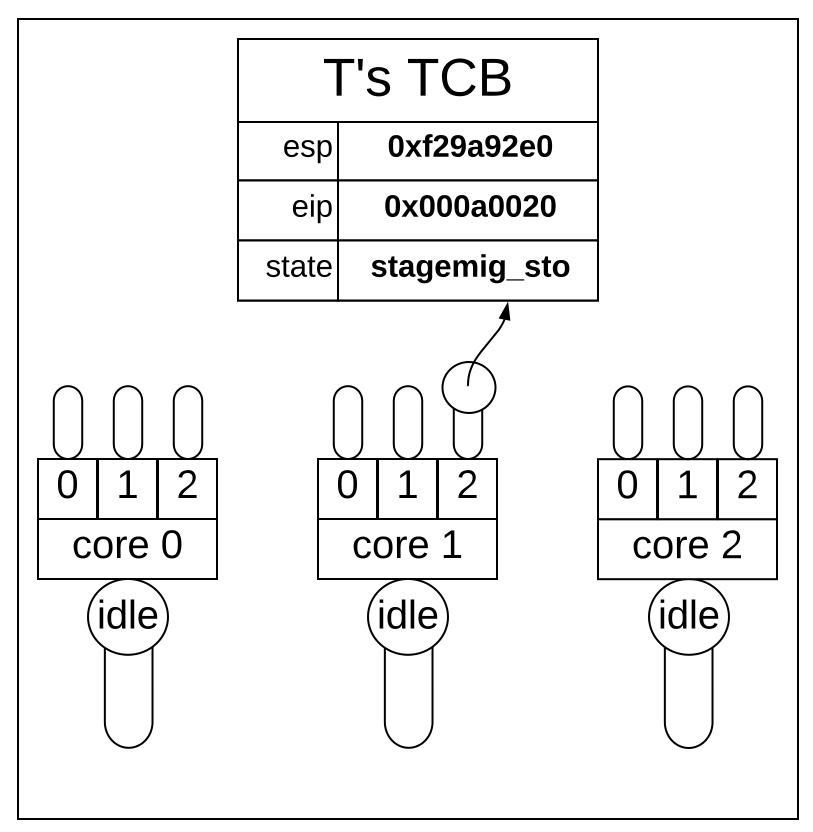
\includegraphics[width=5cm]{fig_build/mig2}
    }
    \hspace{1.2cm}
    \subcaptionbox{The idle thread on core1 observes T in state \lstinline[style=figurecpp]{stagemig_sto} and admits it to the ready queue.}[6cm]{
    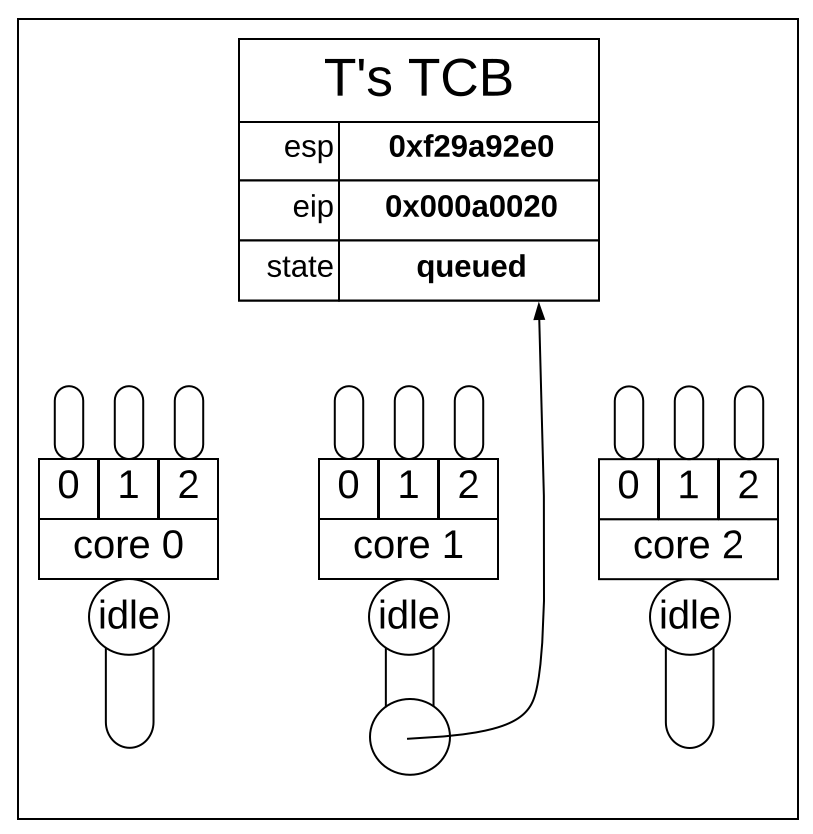
\includegraphics[width=5cm]{fig_build/mig3}
    }
    \hfill
    \par
    \bigskip
    \subcaptionbox{T starts executing on the core1.}[6cm]{
    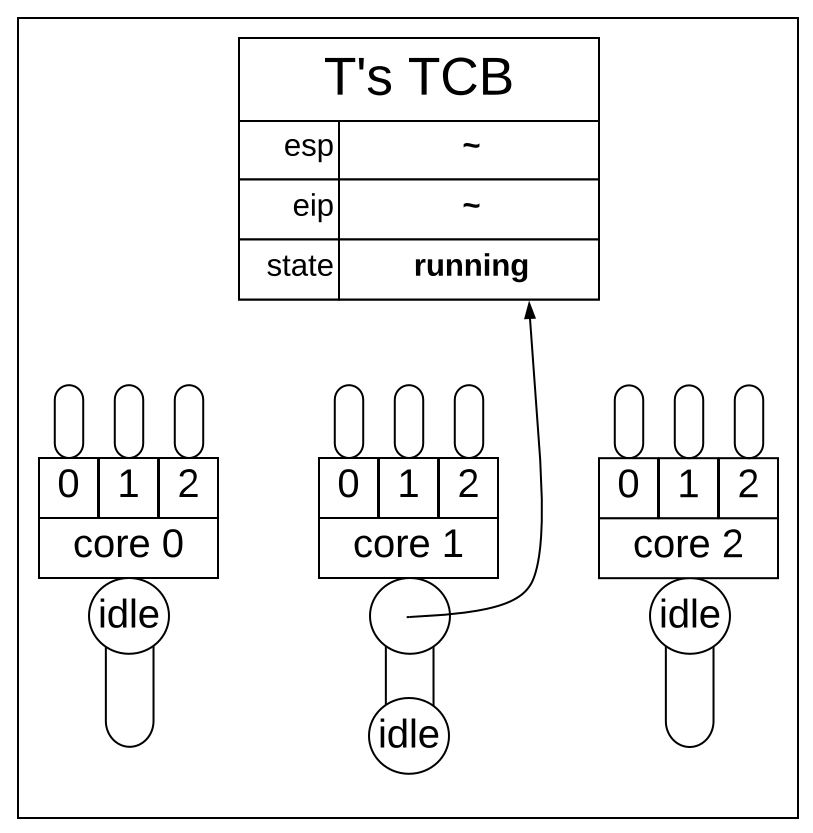
\includegraphics[width=5cm]{fig_build/mig4}
    }
    \caption{Fast thread migration without helper threads.}
    \label{fig:di:mig}
\end{figure}

The other issue we face with our migration mechanism is that in upstream OSv, the idle thread puts CPUs to sleep using the \textsc{\texttt{halt}} instruction.
While this is in upstream due to the use of IPIs which wake the CPU up again, our decision to omit means that we must avoid infinite \textsc{\texttt{halt}}s.
We remove the halting from the idle thread and offer the following alternatives instead:
At first, the idle thread can busy-wait for changes to the incoming migrations queue.
Alternatively, it can use the \textsc{\texttt{monitor}} and \textsc{\texttt{mwait}} instructions to wait for changes to the queue while keeping the core into a low power state.
Both options have benefits and downsides:
Busy-waiting offers significantly lower migration latency (700 -- 800 ns less) \todo{ref eval} but consumes more power, which is undesirable for technical (dark silicon), economical(increased cost) and ecological reasons.
Additionally, SMT machines may see increased performance due to MWAIT because it allows switching to the core's other hardware-thread.~\cite{intelSDMMWAIT,darkSilicon}
%Since our core allocation policy currently does not support SMT \todo{ref limitations / related work} ...

In the last paragraph of this chapter, we want to provide some implementation details that we omitted for easier understanding of the design:
We implemented above mechanism early in the run of this thesis with a limited understanding of the upstream OSv migration mechanism.
We chose to implement our mechanism as a supplement rather than replacement for the upstream version.
As such, the \emph{incoming migrations queue} referred to above is different from the \emph{incoming wakeups} queue from Section~\ref{ch:di:osv:sched}:
Our current implementation uses a lock-free multi-producer-single-consumer queue which we originally used to poll for changes in the idle thread.
The addition of \textsc{\texttt{mwait}} however required waiting for changes to the upstream incoming wakeups queue and our queue simultaneously.
We solved this problem by also setting upstream mechanism's bitmask from the stage-switching code path and by using \textsc{\texttt{mwait}} on its address.
Combined with the changes we present in the next Section, we recommend to merge the two queues and migration strategies and to de-duplicate the dequeuing code.
\todo{out of place?}

The commits in the Git repository corresponding to this section are \refosvcommit{439b55014ea8d3285db7523c4c1ba02b4948cd41} and \refosvcommit{f00b587267797a0bc887243d8cbca661426c8e0b}.

\section{Thread Migration on Wake-Up}\label{ch:di:wake}
% Motivation: with thread migration mechanism in place, we are faster than the Linux solution but not still work conserving
%             when a thread is woken up, it will be enqueued inot the runqueue of the CPU where it went to sleep
%             if that CPU is already executing a thread but another one of the same stage is idle, we do not use the available resources efficiently
%             the woken thread should be migrated to the idle CPU and immediately resume execution there
%             important: this is not stage switching, but also needs to evaluate the CPU allocation policy (forward ref!)
% Design:
%             on wakeup, evaluate the CPU allocation policy and migrate the woken thread to that CPU using the normal thread migration mechanism
% Implementation:
%             wakup is asynchronous, e.g. when from a timer 
%             we must only migrate a thread when it is stopped, otherwise it's already running and does not need to be woken up
%             but there are states in which the thread is being woken up while going to sleep
%             => cleanly encode running vs stopped in the thread state
%               => more difficult than expected
%               => extend post-switch-to mechanism with appropriate state transitions
%               => TODO see git commit
%               => state diagram with changes made in this step
%             Afterwards, just use the existing thread migration mechanism TODO check if we can go without the IPIs
In Chapter~\ref{ch:analysis}, we analyzed that the proof-of-concept implementation in Linux at the KIT OS group is not work conserving:
It only allows thread migration to be initiated from user-space and thus prohibits migrating threads to idle cores at the time the thread unblocks.
In contrast, our solution models stages explicitly and tracks a thread's association with its current stage in the thread's TCB.
Utilizing all cores of a multi-core system is thus trivial in theory:
When a blocked thread is woken up, we find a CPU that has that thread's current stage's code in its cache and enqueue the woken-up thread's TCB into that CPU's runqueue.

However, in practice, this beautiful concept is crushed by the realities of the OSv scheduler implementation.
Let us first look at wakeup-related state transitions that a thread may go through in upstream OSv depicted in Figure~\ref{fig:di:wake:upstreamstates}:
The most common case will be that a thread goes to sleep, waiting on some predicate to become true, for example that a timer has expired or that it aquired a mutex.
The \textit{running} thread will then transition synchronously to the \textit{waiting} state and schedule out.
Let us now imagine that another thread makes the predicate become true.
That \emph{waker} knows the threads waiting for this condition and wakes them using the \lstinline[style=figurecpp]{wake()} function, which puts the woken thread's TCBs into their last core's \lstinline[style=figurecpp]{incoming_wakups}, which is in turn eventually drained into the core's runqueue.

The crucial observation for this section is that the corresponding \textbf{OSv thread states do not precisely encode whether the a thread has stopped executing}.
In fact, only threads in state \textit{queued} are guaranteed to be stopped and only threads in state \textit{running} are guaranteed to be running.
The remaining triad of \textit{waiting}, \textit{sending\_lock} and \textit{waking} is ambiguous:
In each of these states, the thread can either have completed scheduling out or it can still be on the way to do that.
In the latter case, the thread may even observe that it has already been woken up again by some other thread and move itself from \textit{waking} back to \textit{running}.

\begin{figure}
    \centering
    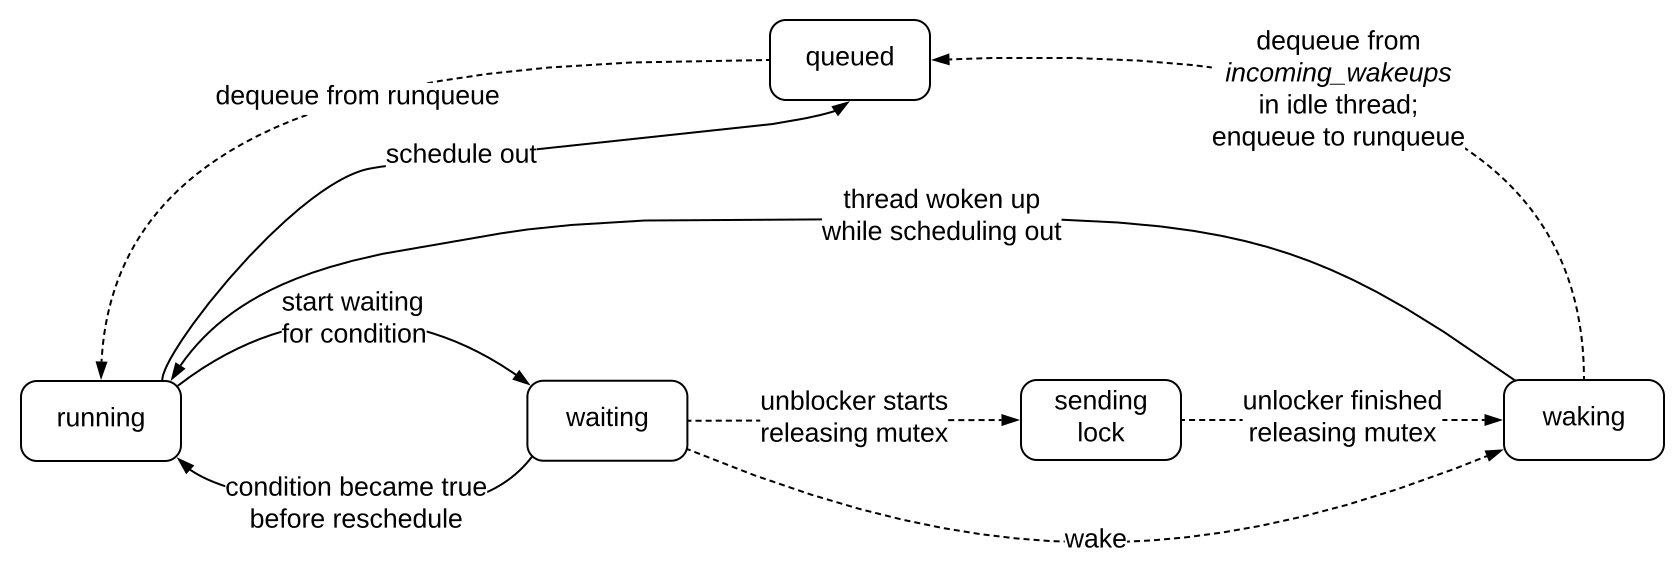
\includegraphics[width=\textwidth]{fig_build/state_chart_pre_spread}
    \caption{Upstream OSv wakup-related thread state transitions: States \textit{waiting}, \textit{sending\_lock} and \textit{waking} are ambigous with regard to whether the thread is still scheduling out whether it has fully stopped executing.
    Dashed lines represent events asynchronous to thread execution, solid lines represent synchronous events.}
    \label{fig:di:wake:upstreamstates}
\end{figure}

Upstream OSv can afford this ambiguous state representation because its wake-up mechanism does nothing but to ensure that the woken thread is made runnable on its current CPU.
\textbf{Our solution however requires precise knowledge of whether the woken thread is still running or whether it has actually stopped executing on its current CPU.}
In the former case, we do not want to migrate it because its current CPU still has a hot cache.
However, in the far more common case of waking up a stopped thread, we want to use the opportunity for load-balancing by migrating the to-be-woken thread to the least-loaded CPU core, thereby maximizing CPU resource usage.
And because the woken-thread is not running at the time of wake-up, we can implement remote asynchronous thread migration that works without a chasing helper thread.

The first pillar of our work-conserving scheduler implementation is therefore a significant refactoring of the OSv thread states:
As we already did with the \textit{stagemig\_run} and \textit{stagemig\_sto} states in Section~\ref{ch:di:mig},
we spread the three \textit{waiting}, \textit{sending\_lock} and \textit{waking} states into \textit{$\star$\_run} and \textit{$\star$\_sto} sub-states; the the former suffix represents a still-running thread while the latter represents a stopped thread.
\textbf{The context switching routine then implements the switch from \textit{$\star$\_run} to \textit{$\star$\_sto} after saving the register state of the thread to its TCB.}%
\footnote{The implementation in the context switching routine is a generalization of the two-step migration mechanism presented in Section~\ref{ch:di:mig}.}
An asynchronous waker can thus always distinguish between running and stopped threads.
Figure~\ref{fig:di:wake:spreadstates} presents the resulting state transition diagram.

\begin{figure}
    \centering
    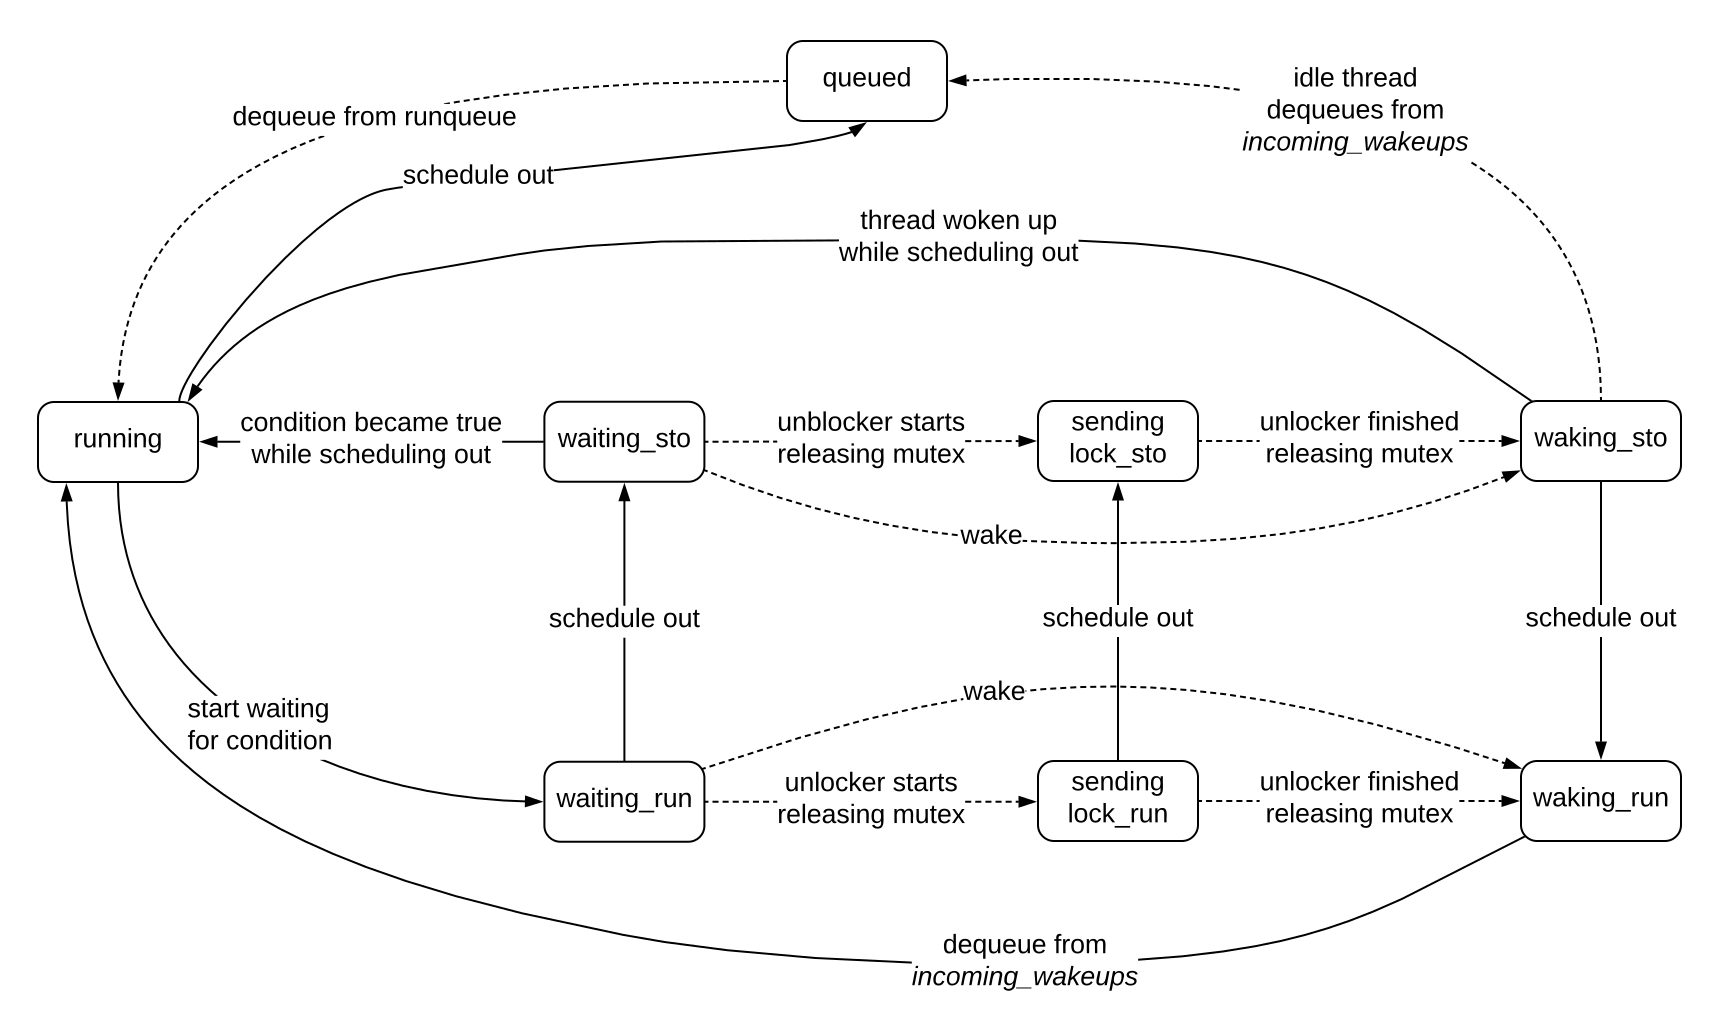
\includegraphics[width=\textwidth]{fig_build/state_chart_post_spread}
    \caption{Modified OSv wakeup-related thread state transitions: All states are unambious about whether the thread is still running or completed scheduling out.
        Dashed lines represent events asynchronous to thread execution, solid lines represent synchronous events.
    }
    \label{fig:di:wake:spreadstates}
\end{figure}

With the refactoring of the thread states done, we can now discuss our faster alternative for remote asynchronous thread migration.
Let us recall some details on upstream OSv from Section~\ref{ch:di:osv:sched}:
\begin{enumerate}[label=(\alph*)]
    \item The waker may run on another CPU than the woken-up thread.
    \item The timer implementation requires all timers of a thread to be on one CPU.
    \item Remote asynchronous thread migration relies on a short-lived helper thread that chases the to-be-migrated thread and eventually performs the same steps required for synchronous thread migration in the name of the to-be-migrated thread.
\end{enumerate}
The helper thread is necessary because the timer implementation only allows suspending timers on the core they would fire on.
Looking at the version control history of upstream OSv, we see that the current timer implementation (commit 786a576e0, 2013) predates asynchronous thread migration support (commit 6bb95442c, 2016).
Furthermore, upstream only requires the latter for the POSIX \lstinline[style=figurecpp]{pthread_attr_setaffinity_np} syscall.
Therefore, we assume that the helper-thread-based solution was considered good enough --- in fact it is a quite elegant engineering trade-off.
However, we require remote asynchronous thread migration to be fast and thus do not want to pay the price of the helper thread.
Also, we cannot afford a remote function call to reprogram the source CPU's LAPIC timer.

Let us therefore reconsider the minimal requirements to make remote asynchronous migration work:
We need a waker $T_w$ on CPU $C_1$ be able to migrate a stopped thread $T_s$ from a remote source CPU $C_2$ to a remote destination CPU $C_3$. $T_w$ must
\begin{enumerate}
    \item remove $T_s$'s timers from $C_2$'s timer list,
    \item put $T_s$'s TCB into the incoming migrations queue of $C_3$ that corresponds to CPU $C_1$ and
    \item set the corresponding bit in $C_3$'s incoming migrations bitmask.
\end{enumerate}
We observe that the timers in step 1 only need to be \emph{removed} remotely and that \emph{resuming} them on CPU $C_3$ is the job of the CPU-local dequeue operation.
We recall that the CPU-local timer lists are sorted ascendingly by expiration date and that the underlying hardware timer is programmed to the expiration date closest in the future.
However, it is not a problem if the hardware timer fires and the corresponding timer object is no longer in the list:
The implementation will simply re-program the hardware timer to the closest timer in the future, i.e., the list head timer's expiration date.
Our solution for remotely suspending timers exploits this property:
We protect each CPU's timer list with a recursive spinlock and extend the timer implementation accordingly.
The waker can then follow the steps described above.
While the source CPU will incur a spurious timer interrupt, we fully avoid all overhead associated with the original helper thread.

After these substantial refactorings, we finally have an efficient way to perform remote asynchronous thread migration in the context of the waker and thus immediately dispatch a woken thread on a suitable CPU core according to the current core allocation.

The relevant commits for this section are \refosvcommit{80d619a810b1e768c49c1acb89ebfbb8a31ecacd} and \refosvcommit{7df1b22f57b8ba90abb4658117599d06620c900a} (state spreading), \refosvcommit{13fbe6743921d9c8308b823a2bb8e21584a09df1} (remotely suspend timers) and \refosvcommit{ed043e94efee8dc4a532f51a46c4a86e7f28778b} (thread migration on wake-up).

\section{Core Allocation Policy}\label{ch:di:pol}
% remove load balancing + fairness (cpu time, priority queue / sorted list? )
% stub out pthreads_sched_setaffinity_np + remove dead thread migration code (why did we do that?)
% implement simple CPU-local non-preeemptive round-robin: non-preemptive is ok because handlers will finish and is good for cache performance (see stagedExecutionDBMS, p5 up left, p10 5.1.2)
% describe outcome:
%   cpu-local runqueues, round robin, non-preemption (OKish because threads always finish, while not really fair...)
%   existing thread migration mechanism still required by percpu threads, but only on startup
%   idle threads are always runnable, dequeue incoming migrations per CPU
%   
%
% TODO read harizopoulos, affninity scheduligng in staged servers and make sure we are not in stark contrast to their results... one argument for that could be that they focus on single CPUs and only have stiefmütterlich solution for mulitple CPUs (see section 6)
% Difference to STEPS: we target multi- to manycore go conceptually, 

% Motivation: bottleneck stages = stages with more-than-avergage threads in the ready queues of processors assigned to these stages
%             natural observation: stage needs more CPU time / cores in our case
%             alterantive formulation (is that correct?):
%                   the time it takes from begin of stage switch to first dispatch on CPU in new stage should be equal among all stages
%                   => predictable latencies
% Design:
%            among all stages, equalize the number of threads that are currently executing / enqueued in each of them
%            why?
%                   => obvious that this eleminiates bottleneck stages
%                   => idea: in systems with #concurrent_requests > #cpus, 
%                   => TODO check queueing theory, would be nice to have some actual formulas here ;)
%
%            equalizing by giving a busy stage more CPUs / taking CPUs from a non-busy stage
%            and between the CPUs assigned to a stage, arbitrate by runqueue length

%              => analogy of requests to be handled = water in pipes...?
%              => a CPU will still have threads from the previous stage in the runqueue: doesn't matter because...
%                    ...they will be migrated off this CPU as soon as they schedule out / block on I/O
%                    ...round robin ensures the caches are warm for the remaining threads in the old stage
%                    ... we know the requests will finish processing eventually

% Design Deficiencies:
%              if the runqueues are long, this system reacts slowy
%                   => would need to migrate runqueue threads off-cpu 
%                       => could do this lazily in schedule()
%
% Implementation:
%               track c_in per stage in atomic counters
%               ... see patch, fairly boring
%               max_stages, snapshot runqueue counters 
Up to this point, we have discussed the two main mechanisms of our design:
We use synchronous thread migration for stage switching and asynchronous remote thread migration for load-balancing thread migration on wake-up.
Also remember that the principal rule of our scheduler is to only dispatch threads on cores that are allocated to the thread's current stage.
Both mechanisms therefore migrate a thread to the least-loaded core in the set of cores allocated to the thread's current stage.
This section now presents the policy used to periodically compute the core allocation.

%Recall that the basic idea of our solution is to dedicate CPU cores and hence their private caches to stages, and only dispatch threads onto those cores that are assigned to the thread's current stage.
%However, in order to fully utilize the available CPU cores, we cannot assume this assignment to be fixed:
%Each thread may thread may spend a different amount of time per stage, either because the stages' code has different fixed runtimes or because their runtime depends on request parameters.
%Therefore, the core allocation policy must be periodically re-asssessed, and the system must support a changing core allocation efficiently.

The basic concept of our allocation policy is simple:
\textbf{We define \emph{stage load} as the number of \emph{runnable} threads in a given stage and dedicate CPU cores to stages proportional to the stages' load.}
After computing a core allocation, we use it to select a target CPU on stage switch and wake-ups (see Sections~\ref{ch:di:mig} and \ref{ch:di:wake}).
If a stage has been assigned multiple CPUs, the CPU with the shortest runqueue is chosen.
Each CPU schedules its runqueue using non-preemptive round robin. \todo{evaluation / discussion}
After a given core allocation has exceeded the boot-time-configurable \emph{maximum assignment age}, we re-evaluate the core-allocation policy using the then up-to-date stage load distribution.
It is crucial to observe that this setup creates a feedback-loop depicted in Figure~\ref{fig:ch:di:pol:feedbackloop}:
The number of cores available to a stage increases the CPU time available to its runnable threads, thereby avoiding that a single stage becomes a point of congestion.
Among the cores of a stage, the load is evenly distributed by always choosing the CPU with the shortest runqueue for migrations.

\begin{figure}
    \missingfigure[figheight=6cm]{feedback loop as in SRT}
    \caption{The basic feedback loop of our core allocation policy: Stage load is defined as the number of runnable threads in a given stage. CPU cores are allocated to stages proportional to the stage's load.}
    \label{fig:ch:di:pol:feedbackloop}
\end{figure}

For a more detailed description of the implementation, let us first summarize the requirements of the rest of the system:
When a thread synchronously switches stages, we need to find a target CPU that is assigned to the target stage.
When waking up a stopped thread, we need to find a CPU that is assigned to that thread's current stage.
While stage switches may be relatively infrequent throughout the handling of a single request, that is not true for wakeups, for example because the request handler performs blocking I/O.
Consulting the core allocation should therefore be fast.
Additionally, all cores use the same core allocation concurrently, but at the same time, our design also involves periodic updating of the assignment.
The update mechanism must therefore be designed to allow all cores to make progress during an update.
Lastly, an update should be minimal in the number of cores that switch to another stage, in order to minimize the sum of capacity misses incured due to the update.

Our implementation is based around the \emph{assignment} data structure which represents a concrete mapping of CPU cores to stages, and the \emph{requirement vector}, which only specifies the number of cores to be assigned to each stage.
On a system with $C$ cores and $S$ stages, a requirement is a vector
    \[ r = \begin{pmatrix} r_1 & r_2 & \dots & r_S \end{pmatrix}\ \text{where}\ r_i \in \mathbb{N}_0 \ \text{and}\  \sum_{i = 1}^{S} r_i  = C. \]
It is important to emphasize that the components of $r$ must be integers, because CPU cores can only be assigned in integer quantities.
A valid assignment $a_r$ derived from $r$ then maps each of the $C$ cores to exactly one stage:
    \[ a_{r} = \begin{pmatrix} a_1 & a_2 & \dots & a_C \end{pmatrix} \wedge \forall s \in 1 \dots S : \vert\{\, i : a_i = s \, \} \vert = r_s \]
When requirements change to $r'$ and we need to update the assignment to $a_{r'}'$, our goal must then be to minimize ${\vert\{\, i : a_i' \ne a_i \,\}\vert}$ because this is the number of cores that incurs capacity i-cache misses due to change of the executed instruction working set partition.

%We compute the requirements vector periodically using the following algorithm:
%Given the current stage load ${l = \begin{smallmatrix}( l_1 & l_2 & \dots & l_C )\end{smallmatrix}}$, we normalize this vector to $\hat{l}$ such that ${\sum_{i = 1}^{S} \hat{l}_i = 1.0}$.
%We then use ${p = \hat{l}}$ as the initial \emph{priority vector} to distribute $C$ CPU cores among the stages:
%At first, we compute ${f = p * C}$, representing the floating-point quantity of CPUs per stage.
%However, we can only assign integer-quantities of CPUs.
%Therefore, we let ${r' \mathrel{+}= \floor{f}}$ and start a new iteration of the loop using ${p = norm(f - \floor{f})}$ and ${C = C - \sum_{i = 1}^{S} \floor{f}_i}$.
%If ${\floor{f} = \begin{smallmatrix}( 0 & 0 & \dots & 0 )\end{smallmatrix}}$, we shift priorities in $p$ from lowest to highest-priority stage such that after at most $C$ iterations, all CPUs are distributed.~\todo{pseudocode?}

We compute the requirements vector as follows:
At first, we gather the current stage load of every stage and build a requirements vector proportional to the load distribution.
To avoid jitter, we then feed this vector through exponentially-decaying moving average filter which advances every time we compute a new core assignment, thus every \lstinline[style=figurecpp]{max_assingment_age} (default: 20ms).
By normalizing the filter result vector to the number of available CPU cores, we get an ideal floating point count of cores to be assigned to each stage.
However, since cores can only be assigned at integer quantities, we perform element-wise integer division on the normalized vector, the divisor being the number of assignable cores.
The integer quotient is then a vector that contains the numbers of directly assignable cores, which we add to the new requirements vector.
The remainders vector in turn contains the left-over fractions of CPU per stage.
We distribute the still unassigned CPU cores by repeating the above procedure with the remainders vector until all cores are assigned.
To ensure that this loop terminates, we prioritize cores with higher fractions of CPU cores.
The algorithm is given in pseudo-code in Figure~\ref{fig:di:pol:reqvectoralg}.

\begin{figure}
\centering
\begin{minipage}{\linewidth}
\begin{algorithmic}[1]
    \setstretch{1.22}
    % Trick with algorithmicx from https://tex.stackexchange.com/questions/113030/indentation-in-the-algorithm-package-after-ensure-require
    \algrenewcommand\algorithmicensure{%
    \makebox[\widthof{\textbf{Require:}}][l]{\textbf{Ensure:}}}
      \Require   \begin{varwidth}[t]{\linewidth}
        \Statex ${l = \begin{pmatrix} l_1 & l_2 & \dots & l_C \end{pmatrix}}$, current stage load vector
        \Statex ${\tilde{l} = \begin{pmatrix} \tilde{l}_1 & \tilde{l}_2 & \dots & \tilde{l}_C \end{pmatrix}}$, exp.-dec. avg. stage load vector
            \strut
               \end{varwidth}
      \Ensure      \begin{varwidth}[t]{\linewidth}
        \Statex $r$, valid requirements vector
          \strut
               \end{varwidth}

    \State $\tilde{l} \gets \alpha * l + (1 - \alpha) * \tilde{l}$ \Comment move exp.-dec. average
    \State $p \gets \tilde{l} \big/ \Vert \tilde{l} {\Vert}_1$ \Comment norm. load, becomes first priority vector $p$
    \State $c \gets C$ \Comment number of cores left to assign
    \State $r \gets \begin{pmatrix}0 & 0 & \dots & 0\end{pmatrix}$
    \While{c > 0}
        \State \textbf{assert} ${\Vert p {\Vert}_1 == 1.0}$
        \State ${f \gets p * c}$ \Comment floating-point core count
        \If{ $\forall i \in 1 \dots S: f_i < 1.0 $ } \Comment priority shifting
            \State $i_{min} \gets \underset{s\,\in\,1 \dots S}{\text{arg\,min}} f_s$
            \State $i_{max} \gets \underset{s\,\in\,1 \dots S}{\text{arg\,max}} f_s$
            \State $p_{i_{max}} \gets p_{i_{max}} + p_{i_{min}}$
            \State $p_{i_{min}} \gets 0$
            \State \textbf{continue}
        \EndIf
        \State ${r \gets r + \floor{f}}$ \Comment assign integer core counts
        \State ${c \gets c - \Vert \floor{f} {\Vert}_1}$ \Comment account for assigned cores above
        \State ${p \gets (f - \floor{f}) \big/  \Vert f - \floor{f} {\Vert}_1 }$ \Comment priority based on remainders
    \EndWhile
\end{algorithmic}
\end{minipage}
\caption{
    The algorithm to compute the requirement vector proportional to stage load.
    From the second iteration on, we distribute cores proportional to the remainders of the previous iteration.
    Note that because ${l_i \ge 0}$, ${\Vert\cdot{\Vert}_1 = \sum_{i = 1}^{S} \vert l_i \vert = \sum_{i = 1}^{S} l_i}$.
}
\label{fig:di:pol:reqvectoralg}
\end{figure}

The \emph{minimal transition} from $a_r$ to $a_{r'}'$ is then implemented by building a delta vector ${\Delta r = r' - r}$:
Negative comonents represent stages with excess cores whereas positive components represent need for cores.
A simple nested loop then re-assigns cores between components of $\Delta r$ and updates the assignment accordingly.
Note that the constraints on requirement and assignment vectors imply that ${\sum_{i = 1}^{S} \Delta r_i = 0}$, guaranteeing that a full transfer is always possible.
The core re-assignment loop prefers to re-assign cores with a lower index in the global list of cores over those with a higher index.
This implies that cores with a higher-index switch stages less often given a stable system load.
The current asymptotic runtime complexity of the loop currently is in $O(S^2 * C^2)$.
However, we did not spend time on searching lower-runtime algorithms and we do expect most applications to have $S \le 8$ and $C \le 32$, which interpolates to $\approx 200us$ runtime, based on the results of the evaluation. \todo{ref evaluation} % (8^2)×(32^2) * (512ns/(3^2 * 6^2))
More importantly, the time spent on the computation is amortized because the result is re-used for the time specified via the \lstinline[style=figurecpp]{max_assignment_age} boot-time parameter.
For future work, it might be worth to investigating more efficent assignment transition algorithms or to consider auto-tuning the \lstinline[style=figurecpp]{max_assignment_age} based on detected system configuration.\todo{leave stuff about complexity in?}

The last problem of the updating procedure is to support concurrent use of the old assignment while computing a new one.
We use OSv's version of read-copy-update~\cite{readCopyUpdate} (RCU) to accomplish this:
When accessing the current assignment through its public getter, we compare the timestamp of the assignment's creation against the current time.
If the \lstinline[style=figurecpp]{max_assignment_age} is exceeded and there is no other thread already computing a new assignment, the calling thread becomes the updater.
RCU allows all other threads to safely use the old assignment until the new one has been computed.

An important detail of the above algorithm is that a core assignment vector that assigns 0 cores to a given stage is valid.
For example, another stage may be assigned all available cores.
However, our stage switching implementation requires a target CPU at the time the thread calls the stage switching API.
In other words: We do not  have a mechanism to queue up threads whose stage has not been assigned a dedicated core.
Our solution in this situation is to always choose the core $C_v$ with the highest index in the global list of cores as the victim core that must incur the i-cache miss for the underloaded stages' threads.
The reasoning behind this decision is that the described situation should be rare in the first place:
If a stage is constantly underloaded, the stage-switching points were likely not chosen for a representative workload.
The idea behind choosing $C_v$ and not, for example, $C_0$, is that the core with the highest index is already advantaged in the \emph{minimal transition} algorithm:
$C_v$ will least frequently switch stages and is therefore best-suited to be penalized with cache-thrashing threads from the underloaded stage.
Validating and improving this workaround is subject for future work.

The initial implementation of the allocation algorithm was commited in revision \refosvcommit{2f2a8628bc927e41d1e194b8495c84eda82b55ef} and refined in \refosvcommit{cf16063beef7573026a543e0ad68dace6a3eff89}.
The requirements vector is computed as described above since revision \refosvcommit{1d3b25957985eb929e26dd956fb038ca6ec71073}.

\subsection{OSv's Page Access Scanner}
During the implementation of the core allocation policy we found that an OSv system thread called \emph{page access scanner} (PAS) consumes significant CPU time.
It is unpinned (not per-cpu) and thus always executes on cpu0 in our solution because we removed the upstream scheduler's load balancing mechanism and only provide stage-aware scheduling to applications, not OSv system threads.

Since the PAS is apparently the only unpinned system thread that consumes significant CPU time, we investigated it more closely:
OSv's main filesystem is a port of the Zettabyte File System (ZFS) which includes its own Adaptive Replacement Cache (ARC).
The OSv page cache uses the PAS thread to inform the ARC about recent usage of file-backed pages by checking and subsequently clearing the page table entries' accessed bits.
The PAS consists of an infinite loop that self-tunes the CPU time it consumes through a target value $t \in [0.1, 20]$:
It scans pages for $t$\% and then sleeps for $1-t$\% of the time it runs, where $t$ depends on a decaying average of the page access rate.
The loop runs at a hard-coded frequency of 1000Hz.
While this value is respected in the formula to calculate the maximum time the PAS may run before going to sleep, changing it affects the effective amount of work done by the PAS:
For example, when choosing 10 instead of 1000Hz as the PAS frequency, each invocation of the PAS can in theory run up to 100 times longer, but since the entire page cache may be scannable in a shorter time, putting the PAS back to sleep early.
As a side-effect, a reduced frequency also lowers the temporal resolution of the page usage data available to the ARC.

Our core allocation policy does not handle this situation well:
We track stage load in the stage switching and the reschedule routines, not by summing up the length of a stage's cores' runqueues.
Any load caused by system threads is thus invisible to our policy, which is generally acceptable because most system threads are per-cpu-threads and usually sleep.
However, the PAS is an exception in this case because it executes only on cpu0 and is invisible in the stage load vector.
Whenever the core allocation policy assigns cpu0 to a stage, that stage's threads compete with the PAS for CPU-time.
%Within a stage, we always enqueue a thread to the core with the shortest runqueue.
%At a high-frequency of PAS invocations (1000Hz), highto a  core load-balance b
Furthermore, the high frequency of PAS invocations (1000Hz) is detrimental to cache performance on cpu0:
The PAS thread's instruction working set is disjoint from the stage threads' working set and given that the latter barely fits the CPU-private cache, the frequent scheduling of the PAS thread causes thrashing of that cache on cpu0.
%At first, we must emphasize that the use of non-preemptive round-robin scheduling per CPU is not problematic because the PAS thread consistently sleeps after less than 500 $\mu s$ of execution.
%However, a file-system intensive application like MySQL drives $t$ toward $20\%$ of targeted CPU time, thus leaving only 80\% of CPU 0's  time to the stage's threads.

We can quantify the above effect using the TPC-C benchmark by running the single-terminal configuration against MySQL on OSv with 1000Hz and 10Hz PAS frequency.
The results are shown in Figure~\ref{fig:ch:di:osvpageaccessscannerbench}:
We observe that our solution experiences a far more significant speedup compared to upstream OSv.
More importantly, the speed-up correlates with an increase in cache hits.
We interpret this as a confirmation of our assumption that the frequent invocations of the PAS thrash the L2-cache of cpu0 and hence lead to frequent eviction of the instruction working set of the stage assigned to that core.

\begin{figure}[h]
\centering
\begin{tabular}{| r | c | c | c | c |}
    \hline
    \text{Build} & \multicolumn{2}{|c|}{Upstream} & \multicolumn{2}{|c|}{Our Solution} \\
    \hline
    Frequency  & req/sec & L2 i-hits & req/sec & L2 i-hits \\
    \hline
    \text{1000 Hz} & 180 & X \% & 150 & X \%  \\
    \hline
    \text{10 Hz} & 225 & X \% & 220 & X \% \\
    \hline
    \hline
    \textbf{Improvement} & \textbf{25\%} & \textbf{X\%} & \textbf{46\%} & \textbf{X\%} \\
    \hline
\end{tabular}
\caption{The effect of changing the PAS frequency on TPC-C throughput and L2 code hit ratio. Speedup in throughput correlates with L2 i-cache hit rate and reduc.}
\label{fig:ch:di:osvpageaccessscannerbench}
\end{figure}

We have considered several approaches to solve the problems of the PAS in the core allocation policy:
At first, one could model cpu0 as a \emph{{50\,--\,80\%} CPU}.
However, this solution is not very general since we lack a precise model for the impact of the cache trashing caused by the PAS.
Furthermore, the current implementation would require many special cases to support CPUs in non-integer quantities.

Another idea is to declare one core as \emph{the thrashing core}, exclude it from the core allocation and use it to run the PAS.
The natural downside of this approach is that, if the PAS does not run 100\% of the time, we waste resources on that core.
A mitigation would be to change the dispatch policy for underloaded stages, i.e., those stages that do not have enough relative load to win a single dedicated CPU core:
In the core allocation policy presented in Section~\ref{ch:di:pol}, we dispatch threads in underloaded stages round-robin over all cores.
With one core selected as the \emph{thrashing core}, we would dispatch those threads on that core, preventing the otherwise negative cache impact on all the other cores which are dedicated to loaded stages.

Finally, we considered defining a dedicated stage for the PAS.
The main problem with this approach is that our concept is designed for many requests per stage.
The fictional PAS-stage however would only ever have zero or one runnable thread, thus likely never win a dedicated core.
Instead, it would be frequently dispatched on a random core and evict that core's stage's working set.
Experiments showed that this option is not worth pursuing without the concept of a \emph{thrashing core}, at which point one could fully fall back to the proposal in the previous paragraph.

\subsubsection{Impact on Evaluation}\label{ch:di:pol:pas:eval}
The primary goal of this thesis is to show that it is possible to implement work-conserving, stage-aware scheduling policy by choosing the right abstractions and mechanisms.
Ideally, the corresponding scheduling policy should be competitive without further modifications to the remaining operating system.
However, the schedule for this thesis did not allow us to solve the problems that the page access scanner poses to our scheduling policy.
\textbf{Therefore, for the entire evaluation, we set the PAS frequency to 10Hz in both upstream OSv and our modified version.}
As described in the previous section, the reduced frequency removes the impact on core allocation and cache thrashing, which is necessary to show the changes to cache behavior caused by our stage-aware scheduler.
Despite the modifications to upstream OSv being technically unnecessary, we consider the comparison between the 10Hz-versions of upstream and our version of OSv to be fair, since both configurations benefit equally from the removed impact of the PAS.
The implementation of a work-around for the PAS is thus left open to future work.


\section{Limitations \& Future Work}\label{ch:di:discuss}
% big picture
%   multi-threaded server => limits to one concurrency model (that is mostly legacy / java apps?)
%   manual placement of migration points: unpublished work at KIT OS group works on automating that workflow
%   migration increases data misses, so i-cache hits + benefits must outweigh them => need apps with execution phase behvaior => mathias' papermigration points at locations misses thread mandatory thread
% sched policy details
%   non-preemptive round robin => server tasks are I/O intensive, will thus necessarily perform blocking I/O. we could implement preemptive to be safe, but we are pretty sure the timer would never fire 
%   policy does not do smoothing in feedback-loop => if we had more time...
%   core allocation does not work well on idle systems => could implement adaptive scheduler, out of scope for this thesis

Core allocation policy does not support SMT. Show that we need to address this explicitly, draft multi-level version of our algorithm, mention MWAIT again.

We require control of the cache state, i.e. vCPUs in uncommon configuration. See Evaluation.
This is not guaranteed in cloud hosting environments and thus limits applicability.. This is not always guaranteed in cloud hosting environment is operational burden 

The two most relevant are a) the opportunity cost of mandatory thread-migration when switching stages and b) data cache misses when stages share data.
More elaborate discussion on design trade-offs is deferred to then end of this chapter and the evaluation.

%In contrast to cohort scheduling, spreading the instruction working set over the private caches allows the code to be cache-resident for the whole time of the CPU core allocation. \todo{possible benefits of this, are there? otherwise, it's part of the break-even calc, see paper}
%The difference to the computation spreading implementation is we do not rely on virtualization hardware features for thread migration and that we allow migration points at arbitrary points in the application instead of just the kernel boundary.
%Unlike STEPS and the proof-of-concept, we do not supplement an unaware kernel scheduler with a user-space model but make stages a first-class concept of the scheduler instead.

Our design is limited to server applications with high instruction cache footprint and a thread-pool or thread-per-request threading model:
related work has shown that high instruction cache miss rates are a performance bottleneck in scale-out applications
and demonstrated lower cache miss rates in the MySQL database server, which follows the thread-per-request model with a pool of pre-spawned threads.
We re-use their tested stage definitions in MySQL \todo{KIT OS group} and focus on the implementation of a work-conserving scheduling policy.
\cite{kanev2015profiling,mysqlThreading}\todo{KIT OS group}

The limited compatibility with threading models is not a major limitation of our design:
our approach aims at reaping the benefits of staged computation in legacy applications that cannot be easily refactored to a staged-computation model.
Thread-pools and per-request threads were the dominant threading model in the last TODO years and are in fact still used in new applications today.
We acknowledge that more recent runtimes with event-driven concurrency or M:N scheduling models are incompatible with our approach, unless programmers manually construct the supported threading models on top of them.\todo{proof}\todo{discussion section?}



\chapter{Evaluation}\label{ch:eval}
In Chapter~\ref{ch:di}, we presented our operating-system-based solution to mitigate the suboptimal cache behavior of multi-threaded server applications:
We provide a system API to define \emph{stages} which represent spans in the request-handling code path whose instruction working set is smaller than the size of a CPU core's private cache.
The OS scheduling policy is aware of these stages and migrates threads to different cores when they switch stages using fast thread migration mechanisms.
By dedicating CPU cores to stages, threads always execute code that is in the private cache, thus avoiding expensive off-core cache or memory accesses.

In this chapter, we evaluate our implementation in the OSv library operating system to validate the following theses:
\begin{enumerate}
    \item Existing applications can adopt our solution with minimal changes required to the existing code.
        We show this by documenting the adoption of the stage API in MySQL v5.6.
    \item Our solution improves relevant performance metrics for these applications compared to upstream OSv and virtualized Linux.
        We show this using industry-standard TPC-C benchmark.
    \item Above performance improvements are due to the stage-aware scheduling technique presented in this thesis:
    \begin{enumerate}
        \item Our solution spreads an application's instruction working set over multiple cores.
            We show this using the top-down performance analysis method and other performance-counter-based metrics.
        \item Our fast thread migration mechanism and migration on wake-up are required for improving net application performance.
            We show this by implementing the stage API in upstream OSv based on the upstream thread migration mechanisms and comparing performance of both sides using fixed core allocation.
        \item Our core allocation policy allocates CPUs proportional to stage load.
            We show this by instrumenting the corresponding code with OSv tracepoints.
        \item Our core allocation policy improves application performance compared to fixed core allocation.
            We show this using TPC-C over a varying the number of concurrent client connections.
    \end{enumerate}
\end{enumerate}

The remainder of this chapter is structured accordingly:
Section~\ref{ch:eval:setup} describes the hard- and software setup common to all measurements presented in this thesis.
Subsequently, we show the adoption of the stage API in MySQL~v5.6 in Section~\ref{ch:eval:stageapi}.
Section~\ref{ch:eval:perf} then presents the MySQL performance comparison using TPC-C.
The remaining sections cover the validation of our design assumptions:
In Section~\ref{ch:eval:spreading}, we show that we successfully spread MySQL's instruction working set over multiple cores.
We show the advantages of our thread migration mechanisms in Section~\ref{ch:eval:mig} isolated from the influence of the core allocation policy.
The core allocation algorithm and its influence on performance is then validated separately in Section~\ref{ch:eval:polidea} and \ref{ch:eval:polperf}.
We conclude with a discusssion of the results in Section~\ref{ch:eval:discuss}.

\clearpage
\section{Evaluation Setup}\label{ch:eval:setup}
% Intel(R) Xeon(R) CPU E5-2618L v3 @ 2.30GHz
%   8 cores, 2 logical processors per core
%   hyperthreading enabled
% 
% Memory Hierarchy: dmidecode
%   Private:
%       32KiB L1-d and L1-i caches
%       256 KiB L2 unified
%   Shared: 20MiB L3, inclusive, 20-set associative


% NOTES
% taskset -c changed it all around, measurement's don't make sense otherwise

% Disabled L2 Prefetching 0x3 to MSR 0x1a4

% TPC-C number of warehouses
We evaluate our solution on a single-socket Intel Xeon E5-2618L v3 CPU.
The system supports simultaneous multi-threading (SMT) with 8 cores, 2 hardware threads each.
The system has 32 GiB of memory consisting of $4*8$ GiB DDR4 DIMMs clocked at 2133Mhz.
The CPU's cache hierarchy consists of a 20MiB shared, inclusive, 20-way set associative L3 cache, private unififed 256KiB L2 caches and private separate 32KiB L1-d and L1-i caches.
All private caches are 8-way set-associative.
We disable SMT via the BIOS because our core allocation policy does not support it. \todo{ref}
Furthermore, we disable all C-states to reduce latency spikes.

We use the Fedora 27 Linux distribution with Linux kernel version 4.13.9 (Fedora package \lstinline[style=figurecpp]{4.13.9-300.fc27.x86_64}) as the machine operating system.
We remove the measurement noise caused by dynamic voltage and frequency scaling by setting the scaling governor to \lstinline[style=figurecpp]{performance} mode and disabling the \lstinline[style=figurecpp]{turbo} frequency range.

Due to the nature of OSv targeting only virtual machines, our evaluation is done using VMs.
For all experiments, we use the Fedora-packaged QEMU 2.10.0-1 software, which in turn uses Linux KVM and thus Intel VT-x for hardware virtualization.
We use the virtio network and disk paravirtualization drivers in OSv.
Disk images are in raw format, located in the host's tmpfs and emulated without caching using pthread-based disk I/O.
We observed heavy cache thrashing when allowing QEMU helper threads on the same cores as the vCPU threads.
To be able to show the changes in cache behavior that can be achieved with stage-aware scheduling, we thus use the following CPU configuration:
We isolate physical cores 2 -- 7 from the Linux scheduler using the \lstinline[style=figurecpp]{isolcpus=2-7} kernel command line parameter.
The VM is then started with 6 virtual CPU cores (vCPUs) and we map each of the QEMU vCPU threads to one of the isolated cores in range 2 -- 7.
The remaining QEMU threads which are used for timers, async-I/O, etc., continue to be dispatched by the Linux scheduler on cores 0 and 1.

The goal of the above setup is to give the guest operating system control of the cache state of its vCPUs.
This is required for our solution because all expected performance benefits are achieved by optimizing cache behavior.
However, we are also unaware of any factors that would disadvantage in the comparisons made in this chapter.

When using Linux as a baseline, we refer to an installation of Debian 9 in a virtual machine configured to start the MySQL 5.6.38 Docker image.
Inside the VM, we bind-mount the MySQL data directory from the ext4-formatted root partition on the emulated HDD.
For all other aspects, the QEMU configuration described above applies.

With regards to OSv, we must emphasize again we had to reduce the frequency of the \emph{page access scanner} (PAS) system thread from 1000Hz to 10Hz (see Chapter~\ref{ch:di:pol:pas:eval}).
To maintain a fair comparison between our solution and upstream OSv with regards the metrics presented in this chapter, we applied this change to both sides.
For all other aspects of the VM configuration, the QEMU configuration described above applies.

For evaluating MySQL, we use the industry-standard TPC-C online transaction processing benchmark~\cite{tpccSpec}.
TPC-C simulates an online transaction processing workload by modelling a retail company with warehouses and distribution districts that handles sales transactions at sales terminals.
While the number of warehouses control the amount of data stored in the database, the number of terminals controls the the number of concurrent clients to the database system.
We use the benchmark implementation provided by the open source \emph{OLTP Benchmark} project at Git revision \texttt{019d9cf} from Februrary 2018~\cite{oltpbench}.
The process of provisioning the database with test data is very time-consuming and not relevant to the benchmarks in this thesis.
Therefore, we re-use a one-time-generated pre-seed with two warehouses.
For the weights of the different TPC-C request types,, we use the default settings in OLTP.

We run the TPC-C benchmark driver from a separate machine (\emph{benchmark machine}) connected to the main machine using direct 10 Gbit/s ethernet.
This allows us to use high numbers of concurrent benchmark clients without influencing the CPU time available to the QEMU helper threads on the main machine's core 0 and 1.
We use a Linux layer 2 bridge device to enable direct connections from the benchmark machine to the virtual machine, thus avoiding most of the overhead of packet filtering on the main machine.

For capturing performance counter data, we use the Linux \texttt{perf} facility in global-monitoring mode on the main machine for CPUs 2-7.
We use the \texttt{ukHG} event modifiers to capture all events that happen on these cores, regardless of whether they execute code of the main-machine's user-space, kernel or in the guest.
We found that without these modifiers, the OSv caused by the application in OSv are not visible because unlike the Linux VM, OSv does not need to change the privilege level when executing application code.
For recording more event types than physical PMUs available on the CPU, we use perf's time-multiplexing feature, which re-programs the PMUs at the host kernel's compile-time configurable \textsc{\texttt{hz}} frequency.
On our host system, this is \texttt{CONFIG\_HZ=1000}.~\cite{perfTimeMultiplexing}

For running orchestrating and scripting the execution of VMs, the OLTP benchmark and perf, and for collecting the benchmark results, we use a self-written benchmarking tool called \texttt{doltp} which can be found in the appendix.

We process the result data using Python, depending on the pandas 0.22 package in combination with numpy 1.14.0, matplotlib 2.1.2 and seaborn 0.8.1.
All graphs and figures in this chapter are rendered reproducibly from the raw data using code in an IPython notebook, which can be found in the appendix.

\subsection{Configurable Idle Strategy in Upstream OSv}\label{ch:eval:setup:idle}

For the upcoming sections, we require further customizations to the idle thread implementation of upstream OSv.
Specifically, we add a kernel command line parameter that allows to select the action taken by the idle thread when there are no other runnable threads in the runqueue.
We provide the following alternatives and will refer to them by name for the rest of this chapter:
\begin{description}[labelwidth=3em,leftmargin=3.5em]
    \item[\texttt{busy}] Busy-waiting for incoming thread migrations in the \lstinline[style=figurecpp]{incoming_wakeups} queue as part of the upstream thread migration mechanism (see Section~\ref{ch:di:osv:sched}).
    \item[\texttt{halt}] The default behavior in upstream OSv: Spin for a short time, then issue the HALT instruction.
    \item[\texttt{mwait}] Instead of using HALT, use MONITOR and MWAIT to wait for changes to the incoming wakeups bitmask. Do not spin before MWAIT.
\end{description}
The difference between \texttt{mwait} and \texttt{halt} is that the latter causes an exit to the hypervisor while the former does not.
To the hypervisor, \texttt{mwait} will thus appear to consume 100\% of CPU time.

Furthermore, only \texttt{mwait} can be used to measure an undistorted top-down top-level breakdown:
Spinning in a tight loop is neither frontend nor backend-bound and will thus inevitably blow up the retired fraction in the breakdown.
An example for the impact of spinning can be seen in Figure~\ref{fig:eval:stageapi:mysqltd}.

When referring to \emph{upstream OSv} without further qualifiers, we mean upstream OSv with the \texttt{halt} configuration.
For top-down comparison, we use \texttt{mwait} in both our solution and upstream.

\clearpage
\section{Adopting the Stage API in MySQL}\label{ch:eval:stageapi}
MySQL is a widely-used open source relational database management system written primarily in C/C++.
While development already started in 1994, the project continues to evolve until today.
The MySQL server provides its services over a custom TCP protocol and supports concurrent clients through thread-based concurrency:
A pool of pre-spawned threads is used to handle incoming connections and additional threads are spawned on demand if the number of concurrent clients exceeds the pool size.
For this evaluation, we use MySQL 5.6.38 which consists of
%cschwarz@i30pc35:[~/osv_upstream/modules/mysql_56/src]: cloc .
%   14808 text files.
%   13966 unique files.
%   10324 files ignored.
%github.com/AlDanial/cloc v 1.72  T=32.70 s (137.4 files/s, 76789.8 lines/s)
%---------------------------------------------------------------------------------------
%Language                             files          blank        comment           code
%---------------------------------------------------------------------------------------
%C++                                   1164         186090         211489         913611
%C                                      517          36569          40480         458542
%C/C++ Header                          1397          51662         115169         206137
more than 1.5 million lines of code.~\cite{mysqlBeginDevelopment,mysqlThreading,mysqlPopularity}

Furthermore, MySQL exhibits the micro-architectural profile of data-center applications observed by \citeauthor*{kanev2015profiling} at Google (see Section~\ref{ch:relwork:profiling}):
As shown in Figure~\ref{fig:eval:stageapi:mysqltd}, 58\% of pipeline slots during a TPC-C benchmark run are frontend-bound, 18\% backend-bound and 5\% lost to bad speculation, leaving merely 20\% of pipeline slots to be actually retired.
Since \citeauthor*{kanev2015profiling} attribute the frontend-boundedness to i-cache thrashing, we also measured L2 cache misses (Figure~\ref{fig:eval:stageapi:mysqll2}):
More than 66\% of private L2 cache misses in both Linux and Upstream OSv are due to code reads.

\begin{figure}
    \centering
    \resizebox{\linewidth}{!}{
        \input{\evalfigpath{mysqlperf_topdown.pgf}}
    }
    \caption{
        Top-down analysis top-level breakdown of MySQL under the TPC-C benchmark.
        The true frontend-boundedness is only visible when removing any spinning, which we did in Upstream OSv.
    }
    \label{fig:eval:stageapi:mysqltd}
\end{figure}

\begin{figure}
    \centering
    \resizebox{\linewidth}{!}{
        \input{\evalfigpath{mysqlperf_miss_distribution_abs.pgf}}
    }
    \caption{
        L2 cache misses of MySQL under the TPC-C benchmark.
        More than 66\% of of cache misses are due to code reads.
    }
    \label{fig:eval:stageapi:mysqll2}
\end{figure}

All of the above makes MySQL a prime example application that could benefit from our solution:
We expose stages to applications via a C++ interface,
the existing MySQL codebase is large and thus not trivially refactorable to the application architectures presented in Chapter~\ref{ch:relwork},
and the threading model is compatible with our solution.
The L2 metrics further support the assumption that MySQL can benefit from spreading its instruction working set over multiple cores.
At last, given the recent trend of deploying applications as virtual appliances, we expect that OSv's strong requirement for this type of deployment is acceptable due to the performance improvements that our solution delivers.

As described in Section~\ref{ch:di:api}, the stage API requires developers to insert stage switching calls into the request-handling code path such that the underlying thread migration spreads the instruction working set over the available CPU cores.
Our initial approach for this task was to read the MySQL source code, starting at the connection handler and figuring out which of the called code modules are large enough to become separate stages.
As a result, we used the RAII-style switching to separate
\begin{itemize}
    \item the code interfacing with the network stack \\ (function \lstinline[style=figurecpp]{do_handle_one_connection}),
    \item the SQL parser (function \lstinline[style=figurecpp]{dispatch_command}) and
    \item the code path handling \textsc{\textit{insert}} queries (function \lstinline[style=figurecpp]{mysql_insert}).
\end{itemize}
The above process was very time-consuming because we were not famliar with the MySQL code base and the resulting throughput measured by TPC-C was too unstable to make it worth pursuing the approach any further.

In parallel to this thesis, staff at the KIT OS group worked on a simulation-based approach to automatically find optimal stage switching points.
At first, a memory access trace is recorded using a full-system simulator while running a representative workload.
In addition to the access trace, a log of the function calls made during each incoming request is made.
The second step is then responsible for finding the optimal position of $N$ stage switching points:
For every combination of $N$ different functions, it replays the memory access trace in a cache simulator and counts the cache misses.
The combination of functions with the minimal number of misses is then chosen as migration points under the assumption that they represent an optimal working set partitioning.
A developer then manually inserts the switching calls directly before the function call.~\cite{kitOSSFMA}

For this thesis, we used the above approach to find an optimal partitioning for 3 stages.
A larger number of stages was impractical due to the runtime of the above algorithm.
The resulting diff statistics are printed in Figure~\ref{fig:eval:api:diffstat}:
The changes amount to 54 insertions and two deletions throughout nine files, and 32 lines of these insertions are isolated in two new files prefixed with \texttt{my\_osv} that contain the declaration and definition of stage pointers as global variables.
This change amounts to only 0.0036\% of the lines of code present in MySQL and is simple to maintain across patch-level changes.
The design goal of a slim stage API can therefore be considered fulfilled.

\begin{figure}
\begin{lstlisting}[style=figurecpp]
git diff --stat 38e2b4d1fe7564b8e1a0d0f0eeb7f542d0d534b6
 CMakeLists.txt            |  5 ++++-
 sql/CMakeLists.txt        |  5 ++++-
 sql/my_osv_stagesched.cc  | 18 ++++++++++++++++++
 sql/my_osv_stagesched.h   | 14 ++++++++++++++
 sql/mysqld.cc             |  5 +++++
 sql/sql_class.h           |  1 +
 sql/sql_lex.cc            |  3 +++
 sql/sql_parse.cc          |  2 ++
 storage/perfschema/pfs.cc |  3 +++
 9 files changed, 54 insertions(+), 2 deletions(-)
\end{lstlisting}
\caption{The Git diff statistics of all changes to upstream MySQL required to insert the stage-switching points computed by simulation}
\label{fig:eval:api:diffstat}
\end{figure}

However, there are a number of obvious points for criticism in the above approach:
At first, the cache-simulator-based switching points are located at semantically unintuitive positions in the source code.
Thus, while the patch is small in size, a human developer can only port it across patch-levels of a given version of MySQL, hoping that the instruction working set does not change significantly.
For a new minor or major version, a one-time re-run of the simulation process would thus be required. \todo{comment on this?}
Secondly, the patches are specific to the simulated cache hierarchy, requiring ready-to-run images to be built per targeted CPU.
While this approach is prohibitive for fragmented setups, we expect the targeted medium to large-scale deployments to use homogenous hardware, facilitating deployment.
Additionally, it should be noted that the very popular Intel x86-64 micro-architectures since \emph{Nehalem} (2008) have used the same cache sizes and associativity per core, although \emph{Skylake} server processors have moved form 256KiB to 1MiB L2 cache in 2017~\cite{nehalemCacheHierarchy,skylakeServerCacheHierarchy}.
Lastly, one can argue that the promised ease-of-use is actually limited by the requirement to use the cache simulator to find switching points.
Indeed, we can imagine a lot of improvements to the tooling but leave this subject to future work.

\section{Whole-System Benchmark with MySQL}\label{ch:eval:perf}
% hypothesis: Stagified MySQL exhibits higher throughput with our scheduler than on upstream OSv and possibly virtualized Linux
%             Stagified MySQL speedup is better with increasing number of concurrent clients (due to reduced i-cache misses, etc)
% method: oltp tpc-c, vary number of terminals => oltp.py, needs re-work to work over multiple machines
%         measure: throughput, maybe latency and response time
%         4-way comparison: our osv + stagified mysql, upstream osv unmodified mysql, vm linux + unmodified mysql, metal linux + unmodified mysql
%         vm image always in ramdisk, linux should use zfs for fair comparison
% discussion: likely metal linux will outperform all vm-based solutions. maybe experiment with network-card passthrough
In this section, we show that stage-aware scheduling is able to improve performance of real-world applications by the example of MySQL, which we adapted to use the stage API in the previous section.
We use the TPC-C benchmark setup as described in Section~\ref{ch:eval:setup} to compare the performance of MySQL running on our solution versus upstream OSv, an equivalent setup in a Linux VM and bare-metal Linux.

For the purpose of this thesis, the aspects of multi-client and multi-core scalability are of particular interest:
MySQL implements thread-based concurrency, i.e., it uses one operating system thread per client connection and relies on the OS scheduler to utilize multiple CPUs effectively.
In Chapter~\ref{ch:relwork}, we have presented related work showing this model's negative effect on cache behavior:
A request handler's instruction working set does not fit into the private cache of an individual core, thus causing cache thrashing and lost performance.
As laid out in Chapter~\ref{ch:di}, our solution avoids this problem, expecting performance gains due to always-warm instruction caches.

The most important performance metrics for a database system under OLTP workloads are \emph{throughput}, measured in completed requests/second, and the \emph{request latency}.
To show the effectiveness of our solution, we measure these metrics over a varying number concurrent client connections (terminals).
For each data-point, we perform 8 40s TPC-C benchmark runs with identical parameters.
We discard the result data of the first and last two seconds to exclude warm-up and tear-down phases of OLTP.
We also vary the \lstinline[style=figurecpp]{max_assignment_age} parameter to experiment with its influence on application performance.

With regards to throughput (Figure~\ref{fig:eval:perf:throughput}), our solution achieves a speedup of up to 22\% at 50 TPC-Terminals.
While upstream OSv throughput is stagnant after the number of terminals exceeds the number of available hardware threads (6 vCPUs), our solution's maximum throughput is achieved at 20 terminals.
The influence of the \lstinline[style=figurecpp]{max_assignment_age} is negligible.
In contrast, the influence of MWAIT vs. busy-waiting is significant:
we achieve more than double the speedup with busy-waiting compared compared to MWAIT.

\begin{figure}
    \centering
    \resizebox{\linewidth}{!}{
        \input{\evalfigpath{3way_tpcc_throughput.pgf}}
    }
    \resizebox{\linewidth}{!}{
        \input{\evalfigpath{3way_tpcc_throughput_speedup.tex}}
    }
    \caption{
        TPC-C throughput of MySQL on upstream OSv vs. our solution.
        The error bars indicate the standard deviation over the 8 benchmark runs per configuration.
        The legend entries in top-to-bottom order correspond to the bars in left-to-right order.
        The table below shows the speedup with upstream OSv as the baseline.
    }
    \label{fig:eval:perf:throughput}
\end{figure}

Response time is much less affected by our solution than throughput, as is shown in Figure~\ref{fig:eval:perf:reqlat}.
Only at very high numbers of concurrent clients do we observe lower response times with our solution compared to upstream OSv.
However, even at 60 terminals, the difference amounts to merely 15ms at mean latencies of 1110ms vs. 1095ms.

\begin{figure}
    \centering
    \resizebox{\linewidth}{!}{
        \input{\evalfigpath{3way_tpcc_reqlatency.pgf}}
    }
    \caption{
        TPC-C request latency of MySQL on Upstream OSv vs. our solution.
        The error bars indicate the standard deviation over the 8 benchmark runs per configuration.
        Note that the y-axis starts at 850 msec.
    }
    \label{fig:eval:perf:reqlat}
\end{figure}

\section{Validation of Design Assumptions}
While the above results show that our solution achieves up to 22\% higher throughput in the TPC-C benchmark,
we must still validate that our design decisions are responsible for these improvements.

In the following subsections, we thus isolate individual aspects of our design and show that they have the intended effect.
In Section~\ref{ch:eval:spreading}, we show that our solution actually spreads MySQL's instruction working set over multiple cores.
Subsequently, in Section~\ref{ch:eval:mig}, we show the influence of fast thread migration and thread migration on wake-up.
Lastly, we validate the behavior of the core allocation policy and evaluate it's influence on application performance.

Given the observation that the \lstinline[style=figurecpp]{max_assignment_age} parameter has negligible impact on throughput, we use the default value of 20ms.
However, we continue to perform measurements with both busy-waiting and MWAIT in the idle thread to find the reason for this parameter's significant influence on throughput.

\clearpage
\subsection{Instruction Working Set Spreading}\label{ch:eval:spreading}
% compare our manually chosen points witht hose from mathias' simulation, same measurements as in microbenchmark above
% tpc-c with single terminal, we only want to show the partitioning works
% mysql in ramdisk 
%MySQL Migration points:
%    manual: why should one use relational operatos? comparibility with staged DBMS paper
%    with mathias' simulation: because it's better, show the advantage => check on mathias' paper once it is published
% alread shown that it's a problem in DBMSs, see 'affinity scheduling harizopoulos introduction and page 4'
% TODO compare I-cache missesa and mispred branches with Steps and compspr, who claim that, see steps, p2 rechts oben => 30 warehouses!
% steps paper 4.2 intro explains TPC-C
% mentio nwe run on ramdisk, does I/O actually block? how often? 
% der steps graph (figure 7) sieht ziemlich aehnlich aus
To validate our primary design goal of spreading the application's instruction working set over multiple cores,
we use hardware performance counters and the Linux \texttt{perf} utility to capture events on the vCPUs while executing the TPC-C benchmark.
Specifically, we record L2 cache events as well as those events required to compute the top-down analysis top-level breakdown (see Section~\ref{ch:relwork:topdown}).

\begin{figure}[b]
    \centering
    \resizebox{\linewidth}{!}{
        \input{\evalfigpath{wsspread_l2.pgf}}
    }
    \resizebox{\linewidth}{!}{
        \input{\evalfigpath{wsspread_l2_speedup.tex}}
    }
    \caption{
        L2 cache misses of MySQL under TPC-C benchmark with 1 and 50 TPC-C terminals.
        The table below shows the relative amount of code data misses in our solution vs. upstream.
    }
    \label{fig:eval:spreading:l2}
\end{figure}

%However, for a fair comparison with regards to the Top-Down metrics, we must modify the idle thread implementation of upstream OSv:
%The upstream idle thread \textsc{\texttt{halt}}s the vCPU after spinning on the \lstinline[style=figurecpp]{incoming_wakeups} for a short amount of time.
%We found that the exit to the hypervisor caused by the \textsc{\texttt{halt}} instruction adds noticable cache misses that can be avoided by using \textsc{\texttt{mwait}}.
%Pre-halt spinning in turn does not affect L2 metrics but distorts the Top-Down top-level breakdown: It increases the \textit{retired} fraction at the cost of all other fractions, because a tight loop is neither frontend- nor backend-bound and leaves little room for bad speculation.
%For the above reasons, we use \textsc{\texttt{mwait}} in the idle thread and remove the pre-halt, which makes the upstream OSv idle thread equivalent to our solution in \textsc{\texttt{mwait}} mode.

Figure~\ref{fig:eval:spreading:l2}~and~\ref{fig:eval:spreading:td} visualize the results of the above run.
We observe a reduction of L2 code misses per request by up to 65\% while increasing data misses by at most 2\%.
MWAIT vs. busy-waiting does not affect the cache behavior of our solution significantly.
However, we see increased code misses in upstream when using HALT vs. MWAIT and busy-waiting.
Our explanation for this observation is that HALT causes exits to the hypervisor and thus additional code misses.
With regards to single vs. multiple terminals, we see that our solution only shows increased data misses with unchanged code misses.
This is to be expected given that more requests are likely to touch more data in the same time interval, thus inducing capacity misses.
Upstream shows a reduction in code misses with multiple terminals, which is likely due to code sharing between threads scheduled on the same core.

%We will show in Section~\ref{ch:eval:mig} that busy-waiting reduces migration latency in the upstream mechanism, but since the uptream OSv scheduler only uses migration for load balancing, this change does not influence cache behavior.

For the top-down top-level breakdown, we compare MWAIT remove all spinning from the idle thread by using MWAIT in both upstream and our idle solution's idle thread.
This is necessary because spinning naturally blows up the retiring fracting fraction because a tight loop is neither frontend nor backend-bound.
The results are depicted in Figure~\ref{fig:eval:spreading:td}:
Up to 27 percent points from \textit{frontend-bound} and 1 percent point from \textit{bad speculation} shift to the \textit{backend-bound} and \textit{retiring} category.
As explained in Section~\ref{ch:relwork:topdown}, this is expected given the reduction in L2 code misses.

\begin{figure}
    \centering
    \resizebox{\linewidth}{!}{
        \input{\evalfigpath{wsspread_topdown.pgf}}
    }
    \resizebox{\linewidth}{!}{
        \input{\evalfigpath{wsspread_topdown.tex}}
    }
    \caption{
        Top-down analysis top-level breakdown at 15 terminals using MWAIT in the idle thread.
    }
    \label{fig:eval:spreading:td}
\end{figure}

We interpret the above results as confirmation that we successfully spread the instruction working set of MySQL over multiple cores.
The use of MWAIT does not correlate with the cache behavior of our solution, i.e., the quality of instruction working set spreading is independent of the sleeping strategy.

\clearpage
\subsection{Thread Migration Mechanisms}\label{ch:eval:mig}
% hypothesis: thread migration on Linux and upstream OSv is not faster than 9 - 14 us (ref sodaspr / compspr)
%             our thread migration is as fast as the code path from enqueue to switch_to + memory latency / cache coherence protocol
% method: microbenchmarks using std::clock* which uses high-res clock
%         implement strategy-like, i.e. one strategy using osv api, one using sched_setaffinity (latter should work on OSv and on Linux)
%         5-way comparison (our osv without mwait, our osv with mwait (TOOO patch from mathias), upstream osv, linux 4.*, linux 2.*)
%         histogram
% visualization: bars with box-plot features => histogram
% result: is faster, we know that
% interpretation: mwait costs approx 1us more than busy-waiting, linux 4.* is faster than 2.* because it uses monitor & mwait instead of IPIs on supported platforms

The analysis in the previous section shows that we are successfully spreading the instruction working set of MySQL.
We accomplish this by using thread migration, for which we implemented a mechanism that we claim to be faster than the upstream OSv facility (see Section~\ref{ch:di:mig}).
Additionally, we refactored the wake-up mechanism to allow thread migration on wakeup, enabling immediate dispatch of woken up thread to any of its current stage's cores (see Section~\ref{ch:di:wake}).
In this section, we validate that we reduced migration latency, the effect of this change on throughput and the additional speedup achieved through thread migration on wakeup.

As a baseline for comparison, we implement the stage API in upstream OSv using the upstream thread migration primitives:
Specifically, we disable the load balancing mechanism and implement thread migration on stage switch using the \lstinline[style=figurecpp]{thread::pin(thread*, cpu*)} remote asynchronous thread migration API.
We cannot not use the synchronous API (\lstinline[style=figurecpp]{thread::pin(cpu*)}) for this purpose because it reproducibly crashes with failed assertions in the upstream timer implementation when invoked at high frequency.
We configure both upstream and our solution to use fixed core allocation with two dedicated cores per stage.
Both implementations choose the core with the shorter runqueue length as migration target.
In addition to the configurable idle strategies in Section~\ref{ch:eval:setup:idle}, we also implemented an option to disable pre-halt spinning in the idle thread.
For brevity, we will refer to the pre-halt / pre-mwait spinning as \texttt{prespin} and for direct halting / mwait as \texttt{nospin}.

We measure stage switching latency using a self-written micro-benchmark (\texttt{hopper}).
We configure the benchmark to define 3 stages and perform 100000 round-robin stage migrations.
\texttt{hopper} discards the first 1000 iterations and collects the remaining results in a histogram with 200ns buckets.
Figure~\ref{fig:eval:mig:hopperdists} shows the results:
Our solution achieves a mean latency of 1300ns with more than 97\% of migrations under 1400ns.
The influence of MWAIT is visible in form of a slightly wider-spread distribution and an increased mean value 1660ns, amounting to 260ns additional latency.

Upstream OSv achieves 6146ns mean latency in the \texttt{mwait-nospin} configuration and 6528ns in \texttt{halt-nospin} configuration.
As can be seen in the histogram, \texttt{mwait-prespin} and \texttt{busy} achieve practically equivalent latencies at $\approx$ 4300ns while the \texttt{halt-prespin} configuration has approximately the same offset to \texttt{mwait} in the \texttt{nospin} case.
For the micro-benchmark, this is unsurprising, because it does not perform any work in a stage, switching to the next one immediately.
Apparently, the benchmark reaches the first stage again before both of its cores went to sleep.

We were unable to find an explanation for the different penalties of MWAIT for our solution vs. upstream (+260ns vs. +1800ns).
% IPIs are only enabled for HALT, and we tested manually that the addiitonal irq_lock with the lock guard is not causing significant latency
However, the more important observation is that even with busy waiting, our solution has more than 300\% lower latency.
The mean value of 1660ns with MWAIT is as fast as bare-metal IPIs propagation time.~\cite{ipiLatencyPopcornLinux}
Since busy-waiting in upstream and our solution have the same propagation time through the cache coherence protocol, we can be certain that all additional overhead is due to interrupt virtualization and the performance implications of helper threads in upstream OSv.

\begin{figure}
    \centering
    \resizebox{\linewidth}{!}{
        \input{\evalfigpath{threadmig_hopper_hists.pgf}}
    }
    \caption{
        Histogram of \texttt{hopper} migration latencies with 200ns buckets, bars drawn at the center of each bucket.
        The last row shows the exact mean values.
    }
    \label{fig:eval:mig:hopperdists}
\end{figure}

Despite the insights presented above, we must still investigate whether the reduced migration latency has any practical effect on application performance when using thread migration for spreading the instruction working set.
To measure this, we use the TPC-C benchmark with a single terminal and compare the achieved throughput.
The absence of concurrent clients removes the influence of thread-migration on wake-up and allows us to attribute speedup solely to faster stage switches.
To show the additional speedup due to thread-migration on wake-up, we then repeat the above experiment with more than one terminal.

The results are presented in Figure~\ref{fig:eval:mig:tpcc}:
With a single terminal, our solution achieves 8 -- 10\% increased throughput compared to all upstream configurations.
With regards to the influence of busy-waiting vs. MWAIT, we see a 14\% increase for our solution with busy-waiting and a single terminal.
For upstream OSv, throughput for a single terminal is not affected by pre-spinning vs. directly going to sleep.

For an increased number of terminals, we observe that our solution maintains an 8 -- 10\% speedup with MWAIT, and gains another 10 percent points when using busy-waiting. Our interpretation is th
We attribute this extra these extra 10 percent points to thread-migration on wakeup.

Additionally, we observe that upstream achieves similar performance with pre-spinning-then-halt vs. busy-waiting.
This means that during the benchmark, every core is used so frequently that it never goes to sleep.
When further comparing the pre-spin to the no-spin configuration, we observe a performance gap of up to 90\% for high terminal counts.
The gap for our solution is only 10\%, which we see by comparing the bars in the left and right column of the figure.
The data does not allow us to distinguish between the influence of reduced migration latency and thread migration on wake-up in this case.

\begin{figure}
    \resizebox{\linewidth}{!}{
        \input{\evalfigpath{threadmig_tpcc_throughput.pgf}}
    }
    \hfill
    \par
    \hspace{1.5cm}
    \resizebox{0.65\linewidth}{!}{
        \input{\evalfigpath{threadmig_tpcc_speedup.tex}}
    }
    \caption{
        TPC-C throughput achieved with fixed core allocation over varying number of terminals.
        The error bars represent standard deviation.
    }
    \label{fig:eval:mig:tpcc}
\end{figure}

\clearpage
\subsection{Core Allocation --- Validation of Implementation}\label{ch:eval:polidea}

The last major component of our design is the core allocation policy.
We validate that it works as designed by instrumenting the allocation code with OSv tracepoints, recording the momentary stage load vector, the new core assignment and the total execution time of the core allocation algorithm in nanoseconds.
We use the default \lstinline[style=figurecpp]{max_assignment_age} of 20ms while executing the TPC-C benchmark with 1, 6 and 30 terminals.
The figures referred to in this paragraph present a 1000ms window of a manually captured trace, which amounts to 50 invocations of the core allocation routine.
Since we check relevant data structure invariants at runtime, we will rely on visualizations to validate that the overall idea works as designed.

As can be seen in Figure~\ref{fig:eval:capimpl:cabystageload}, the raw stage load (number of runnable threads per stage) is very spiky and only grows slowly with the number of TPC-C terminals.
As explained in Section~\ref{ch:relwork:concmod}, this pattern is typical for I/O bound servers  --- we assume that MySQL's request handlers frequently switch between runnable and blocked state.
The spiky load legitimates the exponentially-decaying average filter, whose effect can be observed in the first column:
Stage 0 load rises shortly before the 400ms mark but the stage's corresponding entry in the requirements vector only rises from 2 to 3 cores at about 420ms.
Also, we see that the number of cores assigned to a stage only rarely drops to 0.
In combination with the L2 metric results from Section~\ref{ch:eval:spreading}, this confirms that our stage switching points were well-chosen:
All stages are used sufficiently to be assigned at least one core most of the time.

The decisions of the \emph{minimal transition} algorithm are visualized in Figure~\ref{fig:eval:capimpl:cabycore}:
As designed, we only see the cores with a lower index switch stages frequently while cores with a higher index clearly tend to keep the same stage.

At last, we take a look at the runtime of the entire core allocation algorithm in Figure~\ref{fig:eval:capimpl:runtime}:
The runtime is obviously independent of the number of threads in the system (around 1$\mu s$) but shows significant jitter.
Given the fact that the runtime is amortized over 20ms, less than 0.1\% of CPU time will be spent on the scheduling algorithm.
However, we want to emphasize that we did not show the critical $O(S^2 * C^2)$ asymptotic runtime complexity of \emph{minimal transition} algorithm in this section.

\begin{figure}
    \centering
    \begin{subfigure}{\linewidth}
        \resizebox{\linewidth}{!}{
            \input{\evalfigpath{cap_assignment_by_stage_load.pgf}}
        }
        \caption{Stage load and resulting requirements vector over time.}
        \label{fig:eval:capimpl:cabystageload}
    \end{subfigure}
    \par\par\hfill
    \bigskip
    \begin{subfigure}{\linewidth}
        \centering
        \resizebox{\linewidth}{!}{
            \input{\evalfigpath{cap_assignments_by_core.pgf}}
        }
        \caption{Core Assignment over time (time on y-axis).}
        \label{fig:eval:capimpl:cabycore}
    \end{subfigure}
    \par\par\hfill
    \bigskip
    \begin{subfigure}{\linewidth}
        \centering
        \resizebox{0.5\linewidth}{!}{
            \input{\evalfigpath{cap_runtime.tex}}
        }
        \caption{Runtime of the algorithm.}
        \label{fig:eval:capimpl:runtime}
    \end{subfigure}
    \caption{Visualization of the core allocation policy decisions.}
\end{figure}




\clearpage
\subsection{Core Allocation Policy -- Performance Evaluation}\label{ch:eval:polperf}

After having validated that the core allocation policy works as designed in the previous section, we will now evaluate its effect on application performance.
As a baseline, we use our version of OSv with fixed core allocation with two dedicated cores per stage.
We continue to use the length of the runqueue to decide on which core within a stage a thread should be dispatched.
We use the TPC-C benchmark with a varying number of terminals to evaluate MySQL performance and concurrently capture L2 metrics on the vCPUs.
Additionally, we perform two separate runs with MWAIT vs. busy-waiting in the idle thread.
The comparison between fixed core allocation and the core allocation policy is fair with regards to available CPU resources because our stagified version of MySQL uses exactly 3 stages, resulting in two dedicated stages per core.

As is visible in Figure~\ref{fig:eval:capperf:table}, the maximum increase in throughput achieved by the core allocation policy is only 3\%, starting at 25 TPC-C terminals and higher.
Additionally, these 3\% are only reached when using busy-waiting --- the speedup with MWAIT is at most 2\%.
The impact of dynamic core allocation on request latency is negligible.
The L2 cache metrics show that the core allocation policy reduces codes misses per request by up to 5\%.
However, data misses are increased by 1 -- 2\%.

Since these improvements are fairly minor compared to what we saw for fast thread migration in Section~\ref{ch:eval:mig}, it would be rather easy to dismiss dynamic core allocation as unnecessary.
However, we are convinced that the scenario presented in this section is very beneficial to fixed core allocation:
The fixed core allocation is equivalent to the core allocation policy if
\begin{enumerate*}[label=(\alph*)]
    \item the stage switching points are perfectly placed with regards to stage load and instruction working set and \label{ch:eval:polperf:arg1}
    \item the numer of vCPUs is a multiple of the number of stages. \label{ch:eval:polperf:arg2}
\end{enumerate*}
If these two criteria are true, the core allocation proportional to stage load will always result in 2 cores per stage, which is equivalent to the fixed core allocation presented in this example.
We have already shown in Section~\ref{ch:eval:polidea} that our stage switching points are very close to an ideal placement, which is likely due to the simulation-based approach that we used to find them (see Section~\ref{ch:eval:stageapi}).
Because we use 6 vCPUs for 3 stages in MySQL, condition \ref{ch:eval:polperf:arg2} is also true.

\begin{figure}
    \begin{subfigure}{\linewidth}
        \resizebox{\linewidth}{!}{
            \input{\evalfigpath{cap_perf_throughput.pgf}}
        }
        \caption{
            TPC-C throughput. The y-axis is off-set.
        }
        \label{fig:eval:capperf:throughput}
    \end{subfigure}
    \par\bigskip
    \begin{subfigure}{\linewidth}
        \resizebox{\linewidth}{!}{
            \input{\evalfigpath{cap_per_speedup.tex}}
        }
        \caption{Speedups.}
        \label{fig:eval:capperf:table}
    \end{subfigure}
    \label{fig:eval:capperf}
    \caption{Comparison of the core allocation policy vs. fixed core allocation with varying number of terminals and idle thread strategy.}
\end{figure}

\clearpage
\section{Discussion}\label{ch:eval:discussion}
As shown in in the previous section, our stage-aware scheduling solution is able to improve the throughput of the multi-threaded MySQL database server by up to 22\%.
The speedup is sustained at a high number of concurrent clients.
In contrast to previous work in the field, we do not sacrifice request latency for improved throughput.

At the example of MySQL, we have shown that the required modifications to an existing code base are neglegible to reap the benefits of our solution.
However, we have learned that a simulation-based approach~\cite{kitOSSFMA} for finding stage switching points is preferrable over manual placement by a human developer.

Our thread migration mechanism achieves 1700ns migration latency which is 300\% faster than the corresponding upstream OSv primitive.
The lower overhead of our mechanism is responsible an 8 -- 10\% speedup in throughput with a single client compared to an implementation based on upstream thread migration.
Additionally, we achieve another 10 percent points by implementing thread migration on wakeup for our scheduling policy, thereby overcoming the limitations of the KIT OS group's proof of concept implementation in Linux.

We have shown that our dynamic core allocation policy works as designed by analyzing traces of the allocation algorithm.
The performance evaluation has shown that for our benchmark scenario, the contribution of dynamic core allocation to the total speedup are only 2 -- 3\% percent points.

While this chapter has shown that our design works as intended and that it improves net application performance, the core allocation policy requires further evaluation.
For future work, we plan to conduct experiments using different load profiles and less-optimal stages switching points as well as different CPU configuration.
Additionally, a mathematical model of the opportunity cost of thread migration vs. incuring i-cache misses would help to define an optimal core allocation policy.
The optimal policy would then serve as a scale for evaluating real policies.

\chapter{Conclusion}\label{ch:concl}

In this thesis, we have presented a scheduler design that leverages fast thread migration to spread a multi-threaded server's instruction working set over the private caches of an SMP system.
Our implementation in the OSv library operating system and the evaluation with the MySQL DBMS show that our technique causes a 22\% increase in throughput due to reduced instruction cache misses.

We have shown that previous work in the field unnecessarily trades off request latency for throughput by batching requests to achieve the re-use of warm i-caches.
We argue that these designs are outdated due to the ubiquitous availability of SMP systems, enabling techniques such as computation spreading.
We have presented the groundwork for our thesis done at the KIT OS group:
A software-only approach for computation spreading implemented as a prototype in Linux allows applications to partition a thread's instruction working set at arbitrary points.
By migrating threads to different cores at these points, the instruction working set is spread over the private i-caches of all cores and i-cache misses are reduced.

Our contribution is an analysis of the root cause for the lack of multi-score scalability in the Linux prototype,
the definition of clean OS abstractions for the concept of computation spreading and
a thread scheduler design that is work-conserving.
We define stages as operating system objects that represent spans in the code path of a server application's request handler threads.
Each stage is smaller than the private i-cache of a single core.
We further track a thread's current stage in its TCB, enabling the implementation of scheduler that takes cache-residency of a thread's instruction working set into account.
Our scheduling policy time-multiplexes cache-residency by dedicating cores to stages for certain time intervals.
The scheduler dispatches a thread in a particular stage only onto those cores that are assigned to its current stage.
This enables threads to benefit from always-warm i-caches.
The evaluation has shown that our fast thread migration mechanisms and the integration of our policy into the wake-up mechanisms are the main contributors for increased application performance and multi-core scalability of the concept.

\section{Future Work}

We have already discussed the limitations of the evaluation in Section~\ref{ch:eval:discussion}.
However, there is also room for improvement in the general design.

First, the evaluation setup with pinned QEMU helper threads is not representative of the current offerings of public cloud hosting providers .
Apart from evaluating other virtualization technologies, we can imagine a hypercall interface to pin QEMU helper threads to specific dedicated vCPUs from within the guest VM.

%\item at ITEC OS Group: automatic profiling \& finding of migration points.

Second, integration of our solution into other languages can be simplified by providing a C-version of our stage API.
This is particularly interesting in combination with Java:
The standard library encourages the traditional thread-based model, to which our solution is applicable.~\cite{javaThreadConcurrency}

Third, our scheduler could be extended to program performance-counters during runtime to measure the net-effect of thread migration, e.g., by monitoring L2 i-cache misses.
Additionally, server applications could inform the scheduler about request completions.
Given a mathematical model of the opportunity cost of thread migration, the scheduler could then use the feedback from above data sources as input to the core allocation algorithm.

Finally, the core allocation policy should be extended to support SMT:
The hardware threads of an SMT-enabled CPU are commonly exposed to the operating system as separate logical CPU cores.
The corresponding topology information, i.e., which of these logical cores belong to which physical cores, can be obtained through corresponding instructions.
Since logical cores share the private cache of the physical core, the core allocation policy would need to assert that all logical cores of a physical core are assigned to the same stage to prevent i-cache thrashing.
We expect the performance impact of MWAIT to be at least mitigated by the above, because MWAIT switches the physical core to the other hardware thread if SMT is enabled.~\cite{intelSDMHyperthreading}


\backmatter

\chapter{Appendix}
\blindtext
\begin{itemize}
    \item Source code and commit history of our modified version of OSv
    \item Source code and commit history of our modified version of MySQL 5.6
    \item Source code and commit history of our microbenchmarks and measurement scripts
    \item Evaluation Hardware Memory Hierarchy Topology Information
\end{itemize}

\cleardoublepage
\phantomsection
\addcontentsline{toc}{chapter}{Bibliography}
\printbibliography

\end{document}
